\documentclass[review]{elsarticle}

\usepackage{lineno,hyperref}
\modulolinenumbers[5]
%\usepackage[margin=2cm]{geometry}
\usepackage[justification=centering]{caption}
\usepackage{subfig}
\usepackage{multirow}
\usepackage{xcolor}
\journal{Pattern Recognition}

%%%%%%%%%%%%%%%%%%%%%%%
%% Elsevier bibliography styles
%%%%%%%%%%%%%%%%%%%%%%%
%% To change the style, put a % in front of the second line of the current style and
%% remove the % from the second line of the style you would like to use.
%%%%%%%%%%%%%%%%%%%%%%%

%% Numbered
%\bibliographystyle{model1-num-names}

%% Numbered without titles
%\bibliographystyle{model1a-num-names}

%% Harvard
%\bibliographystyle{model2-names.bst}\biboptions{authoryear}

%% Vancouver numbered
%\usepackage{numcompress}\bibliographystyle{model3-num-names}

%% Vancouver name/year
%\usepackage{numcompress}\bibliographystyle{model4-names}\biboptions{authoryear}

%% APA style
%\bibliographystyle{model5-names}\biboptions{authoryear}

%% AMA style
%\usepackage{numcompress}\bibliographystyle{model6-num-names}

%% `Elsevier LaTeX' style
\bibliographystyle{elsarticle-num}
%%%%%%%%%%%%%%%%%%%%%%%

\begin{document}

\begin{frontmatter}

\title{Deep Learning for landmarking on morphometry anatomical images}
%\tnotetext[mytitlenote]{Fully documented templates are available in the elsarticle package on \href{http://www.ctan.org/tex-archive/macros/latex/contrib/elsarticle}{CTAN}.}

%% Group authors per affiliation:
%\author{Elsevier\fnref{myfootnote}}
%\address{Radarweg 29, Amsterdam}
%\fntext[myfootnote]{Since 1880.}

%% or include affiliations in footnotes:
\author[labri,itdlu]{Le Van Linh\corref{cor1}}
\ead{van-linh.le@labri.fr}
\author[labri]{Beurton-Aimar Marie\fnref{ba}}
\ead{beurton@labri.fr}
\author[labri]{Zemmari Akka}
\ead{zemmari@labri.fr}
\author[igepp]{Parisey Nicolas\fnref{ba}}
\ead{nicolas.parisey@inra.fr}

\fntext[ba]{both authors contributed equally to this work.}
\cortext[cor1]{Corresponding author} 

\address[labri]{University of Bordeaux, 351, cours de la Libération, 33405 Talence, France}

%% %% or include affiliations in footnotes:
\address[igepp]{UMR 1349 IGEPP, BP 35327, 35653 Le Rheu, France}
%% \ead[url]{www.elsevier.com}
\address[itdlu]{Dalat University, Dalat, Lamdong, Vietnam}

\begin{abstract}
Deep learning has been introduced in the middle of the previous century for artificial intelligence, and in recent years, it has risen strongly because of improvements in the computation performance. It has been applied to solve the problems in different domains such as computer vision, speech recognition, or languages translation. Among different types of deep learning architectures, convolutional neural networks have been most often used in computer vision for image classification, object recognition, or key points detection and they have brought amazing achievements. In this work, we propose a convolutional neural network model to predict the key points (landmarks) on 2D anatomical biological images, specifically beetle's images. Our proposed network is trained and evaluated on a dataset including the images of $293$ beetles. During the experiments, the network is tested in two ways: training from scratch and applying fine-tuning process. The quality of predicted landmarks is evaluated by comparing with the manual landmarks which have been provided by the biologists. The obtained results have been considered by the biologists statistically good enough to replace the manual landmarks for the different morphometry analysis.
\end{abstract}

\begin{keyword}
Deep learning \sep CNN \sep fine-tuning \sep landmarks
\end{keyword}

\end{frontmatter}

\linenumbers

\section{Introduction}
\label{sIntroduction}
Deep learning is a part of machine learning domain. Computational model of deep learning is composed of multiple layers to learn the representation of data. Each layer extracts the representation of input data which comes from the previous layers, then it will compute a new presentation for the next layer. In a deep learning model, each layer may contain different number of nodes, called \textit{neurons} which have been inspired from the biological neural system, and the computation at each layer is made by own neurons. Currently, deep learning has many kind of variant architectures and each of them has found success in different domains, i.e. Deep Neural Network (DNN) can be applied to solve the classification or data analysis problems; Convolutional Neural Network (CNN) is widely applied in computer vision, while Recurrent Neural Network (RNN) give the best perform on language modeling.

In deep learning architectures, CNN is a specific network for pre-processing data which have grid topology, i.e. time series (1-D) or images (2D). A CNN consists of an input, an output layer, as well as one or multiple hidden layers. An input after being put on the network will be passed through a series of hidden layers before giving the outputs at the last layer. The computing of CNN affects on $3$ dimensions of data: width, height, and depth. From the first architecture \cite{lecun1998gradient} until now, many CNN architectures have been proposed and have succeeded in different tasks of computer vision such as image classification \cite{lecun1998gradient, krizhevsky2012imagenet,szegedy2015going}, object recognition \cite{szegedy2015going,farabet2013learning,li2015convolutional}.

In computer vision, key points detection is an important field in image analysis. In this field, the algorithms try to find the key points (called interest points or landmarks) in the image. The landmarks are considered as the points in the image that are invariant when the image change i.e. by rotating or translating. Depending on the object, the number of landmarks may be different, as well as their position can be defined along the outline of the object or inside the object. The detected key points are then used in different objectives of different domains, for example, they are fundamental to detect the human face or human pose; in biology, the topography of the objects of an organism can be measured from the location of landmarks. The emergence of deep learning has seen success in other fields of computer vision and key points detection is also not an exception. It has been used to predict the fashion landmarks \cite{liu2016fashion}, human facial key points \cite{sun2013deep,zhang2014facial}, or ear landmarks \cite{cintas2016automatic}.
 
%Key points detection has a wide use and becomes a critical in image analysis of different domains, such as: In geosciences, the key points can be used to recognize the seabed by extracting and comparing the landmarks from sonar images at different times; or computer vision, they are fundamental to detect the human face or human pose; in biology, the topography of the objects of an organism can be measured if we have enough the number of landmarks. Landmarks, or \textit{key points}, or \textit{points of interest}, are the points on the image that store important information about the shape of the object, \textit{for example}, the left and right corners of eyes are two important points to detect the human eyes. Depending on the object, the number of landmarks may  be different, as well as their position can be defined along the outline of the object or inside the object, i.e. the landmarks on Drosophila wings \cite{drosophilaWings} are stayed on the veins of the wings, but the landmarks on human ears \cite{cintas2016automatic} can be located on the ear edge or inside the pimas of the ears.

%Early methods \cite{lowe2004distinctive,bay2006surf,palaniswamy2010automatic} mainly focused on the low level-vision of the image by applying the image processing techniques, and segmentation is most often the first and the most important step in the process. This task remains a bottleneck to compute the features of the complex image. Even if the interested object is easy to extract, the process may take a bit of time to extract the exciting features. The emergence of deep learning has seen success in other fields of computer vision and key points detection is also not an exception. It has been used to predict the fashion landmarks \cite{liu2016fashion}, human facial key points \cite{sun2013deep,zhang2014facial}, or ear landmarks \cite{cintas2016automatic}.

In this work, we propose a CNN to predict the landmarks on biological anatomical images. The proposed model will be trained on the dataset including the images which are taken from $293$ beetles. We will also present another procedure to augment the dataset, which is considered as modest in our case. The predicted landmarks will be provided to the biologists and will be considered to replace the manual landmarks.

%For each beetle, the biologists have taken images of five parts: \textit{left and right mandibles, head, elytra, and pronotum} (Fig. \ref{figbeetles}). All the images are presented in the RGB color model with two dimensions. Along with each image, a set of landmarks has been marked by experts which can be used as ground truth to evaluate the predicted landmarks. During the experiments, the proposed network has been trained on the dataset by applying two strategies. In the first strategy, the network is trained from scratch on each dataset; while in the second strategy, the training process has been modified to include a fine-tuning \cite{yosinski2014transferable} stage. Besides, the value of Root Mean Square Error (RMSE) is used to compute the losses during two experiment processes.

%In some cases, the interested object is easy to extract and can be analyzed by applying the well-known image analysis procedures. Nevertheless, we can not apply the same procedure for un-segmentable images. It really becomes a challenge on the complex images. Luckily, the appearance of deep learning has seen huge success in handwritten digit recognition, speech, images classification and detecting objects in images. Now, an interesting thing is how to use deep learning for landmark detecting, which can be considered as the local characteristic of the image. Our motivation to design a CNN model that able to extract the landmarks on images (even it is segmentable or un-segmentable), which will be used to replace for the previous procedures.

%The main idea consists of the designing and training a CNN \cite{lecun2010convolutional} on a dataset with manual landmarks. Like other CNNs, the features are extracted by using a group of different layer types (i.e. convolutional layer, pooling layer,\ldots) followed by some dense layers to provide the prediction of the network. After designing, the proposed model will be trained on the dataset includes the images which are taken from $293$ beetles. For each beetle, the biologists have taken images of five parts: \textit{left and right mandibles, head, elytra, and pronotum} (Figs.\ref{figh1}, \ref{figt1}, \ref{fige1}, \ref{figlm1}, \ref{figrm1}). All the images are presented in the RGB color model with two dimensions. Along with each image, a set of landmarks has been marked by experts which can be used as ground truth to evaluate the predicted landmarks (Figs.\ref{figh2}, \ref{figt2}, \ref{fige2}, \ref{figlm2}, \ref{figrm2}). During the experiments, the proposed network has been trained on the dataset by applying two strategies. In the first strategy, the network is trained from scratch on each dataset; while in the second strategy, the training process has been modified to include a fine-tuning \cite{yosinski2014transferable} stage. Besides, the value of Root Mean Square Error (RMSE) is used to compute the losses during two experiment processes. For more information about the model, you can see at our repository on GitHub: \texttt{https://github.com/linhlevandlu/CNN\_Beetles\_Landmarks}.
\iffalse
\begin{figure}[htbp]
    \centering
    \subfloat[Head]{\label{figh1}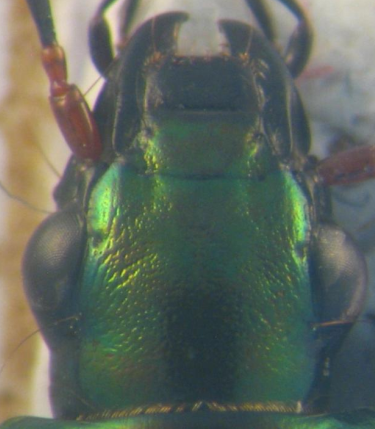
\includegraphics[width=0.3\textwidth]{images/orgHead}}~~
\subfloat[Head's manual landmarks]{\label{figh2}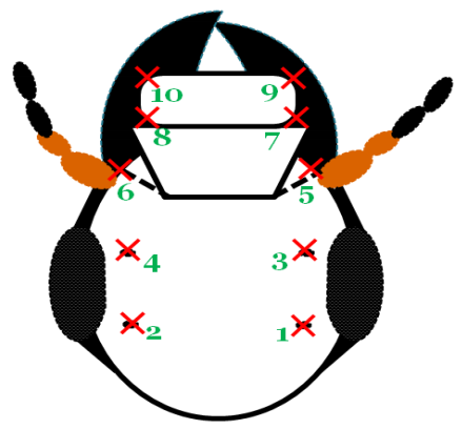
\includegraphics[width=0.35\textwidth]{images/lmHead}}  
    \caption{The \textbf{head} anatomical of beetle and its manual landmarks}
    \label{figbeetle1}
\end{figure}
\begin{figure}[htbp]
    \centering
\subfloat[pronotum]{\label{figt1}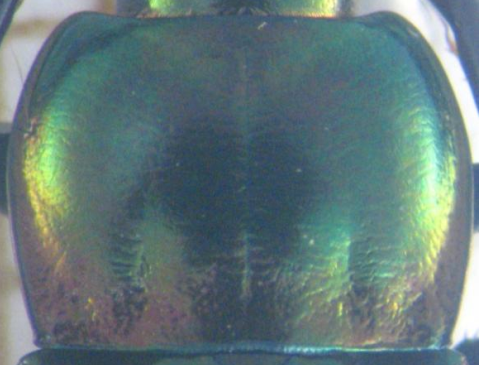
\includegraphics[width=0.4\textwidth]{images/orgThorax}}~~
	\subfloat[pronotum's manual landmarks]{\label{figt2}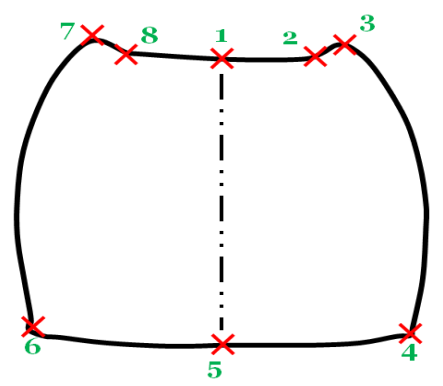
\includegraphics[width=0.4\textwidth]{images/lmThorax}}
    \caption{The \textbf{pronotum} anatomical of beetle and its manual landmarks}
    \label{figbeetle2}
\end{figure}
\begin{figure}[htbp]
    \centering
	\subfloat[Elytra]{\label{fige1}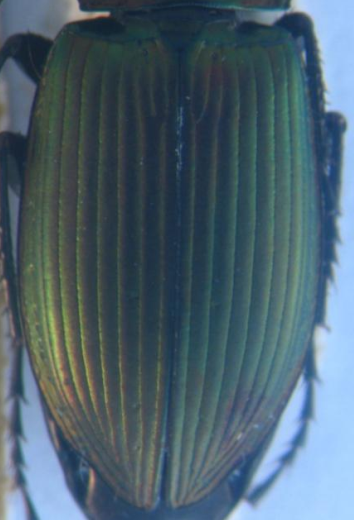
\includegraphics[width=0.3\textwidth]{images/orgElytra}}~~
\subfloat[Elytra's manual landmarks]{\label{fige2}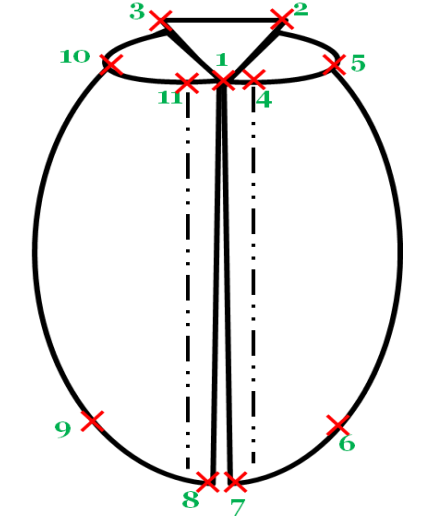
\includegraphics[width=0.35\textwidth]{images/lmElytra}}  
    \caption{The \textbf{elytra} anatomical of beetle and its manual landmarks}
    \label{figbeetle3}
\end{figure}
\begin{figure}[htbp]
    \centering
\subfloat[Left mandible]{\label{figlm1}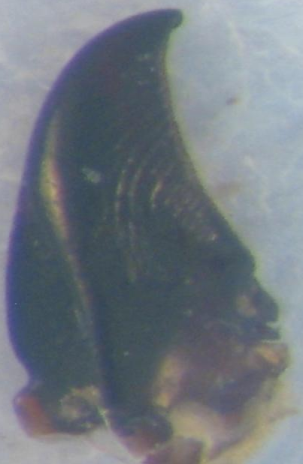
\includegraphics[width=0.25\textwidth]{images/orgLMandible}}~~
	\subfloat[Left mandible's manual landmarks]{\label{figlm2}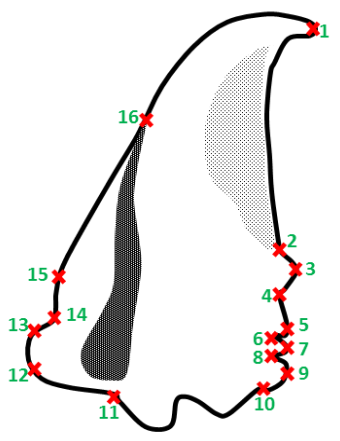
\includegraphics[width=0.3\textwidth]{images/lmLMandible}}    
    \caption{The \textbf{left mandible} anatomical of beetle and its manual landmarks}
    \label{figbeetle4}
\end{figure}
\begin{figure}[htbp]
    \centering
\subfloat[Right mandible]{\label{figrm1}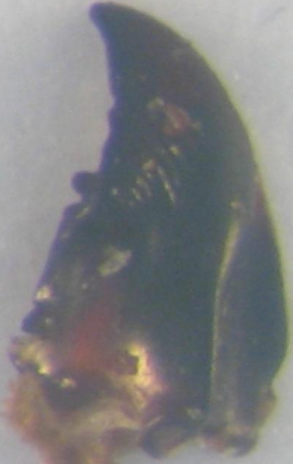
\includegraphics[width=0.25\textwidth]{images/orgRMandible}}~~
	\subfloat[Right mandible's manual landmarks]{\label{figrm2}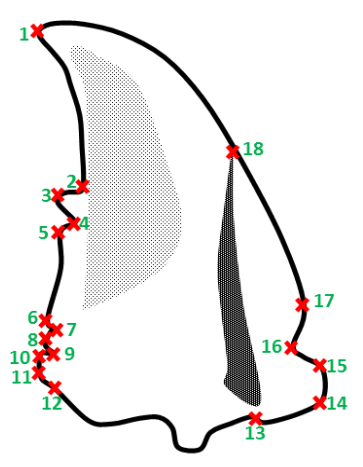
\includegraphics[width=0.33\textwidth]{images/lmRMandible}}    
    \caption{The \textbf{right mandible} anatomical of beetle and its manual landmarks}
    \label{figbeetle5}
\end{figure}
\fi
The rest of this paper is organized as followed: Section \ref{related_works} discusses the related works about determing the landmarks on 2D images. Then, a short overview about CNN and its components will be introduced in Section \ref{sOverview}. Section \ref{Sdataaug} gives another approaches to augment the dataset. Section \ref{Sneuralnetwork} shows the procedure of designing the network model. The first experiment of the network on each dataset is presented in Section \ref{sexperiments}. Section \ref{sfineTuning} presents a modification of training process and its experiment on datasets. Finally, the conclusion is given in Section \ref{sconclusion}.

\section{Related works}
\label{related_works}

In the middle of the previous century, deep learning \cite{lecun2015deep} have been introduced as a method for artificial intelligence applications. However, several problems have appeared when taking into account it into real-world cases because of the limiting of memory or computing time. Nowadays, the improvement of computing capacities, both in memory size and in computing time with GPU programming, has opened a new perspective for deep learning. In recent years, deep learning architectures have achieved remarkable achievements in many tasks of different domains such as \textbf{computer vision} \cite{lecun1998gradient, krizhevsky2012imagenet,  szegedy2015going,farabet2013learning,li2015convolutional}, \textbf{speech recognition} \cite{mikolov2011strategies, hinton2012deep}, \textbf{language translation} \cite{jean2014using, sutskever2014sequence}, \textbf{natural language processing} \cite{lecun2015deep, collobert2011natural, collobert2008unified}, \ldots. In computer vision, deep learning, specifically with CNN, has been used to study the difficult tasks of image analysis such as image classification, or object detection. In the beginning, LeNet \cite{lecun1998gradient} has been proposed and has been considered as the first architecture of CNN. LeCun et al. \cite{lecun1998gradient} have used LeNet in an application to classify the handwritten digits in cheques. LeNet has a standard of a CNN architecture which consists of convolutional layers, pooling layers, then followed by one or more fully connected layers. However, due to the lack of training data and computing power at that time, their network cannot perform the complex problems, i.e. large-scale image, or video classification. From that, many methods have been developed to response the encountered complexity in the training process of CNN. It must take into account AlexNet \cite{krizhevsky2012imagenet}, which has significant improvement upon previous methods on image classification task. Basically, AlexNet \cite{krizhevsky2012imagenet} is similar to LeNet \cite{lecun1998gradient} but it has deeper structure and has been modified some parameters of layers such as using ReLU activation, adding Dropout layer to prevent the overfitting. AlexNet has famously won the ImageNet Challenge \cite{krizhevsky2012imagenet} in 2012. With the success of AlexNet, many models have been proposed to improve the performance of CNN, i.e. ZFNet  \cite{zeiler2014visualizing}, GoogLeNet \cite{szegedy2015going}, VGGNet \cite{simonyan2014very}, or ResNet \cite{he2016deep}. From the comparison of architectures, easy to find that the networks are getting deeper by adding more layers and increasing the depth, e.g. ResNet, which won the champion of ILSVRC 2015, is deeper than AlexNet around $20$ times. Clearly, the deeper models have provided better results but it also increases the complexity of the network, which makes the network be more difficult to optimize and easy to get overfitting.

%Deep learning \cite{lecun2015deep} has been introduced in the middle of the previous century for artificial intelligence application but it has encountered several problems to take real-world cases such as memory or computing time. Luckily, the improvements of computing capacities, both in memory size and in computing time with GPU programming, have opened new perspective for deep learning. In recent years, deep learning architectures are known as the solutions for the tasks in computer vision. Especially in image analysis, CNNs, which consist of convolutional layers, pooling layers, full connected layers, are used to solve the classification or recognition tasks. For example, LeNet \cite{lecun1998gradient} has been known as the first architecture of CNN to read the zip codes and digits. It had a standard structure stacked convolutional layers (normalization and max-pooling) are followed by one or more full-connected layers. From this architecture, many models have been proposed to improve the accuracy as well as computing times in recent years. That must be mentioned to AlexNet \cite{krizhevsky2012imagenet}, ZFNet \cite{zeiler2014visualizing}, GoogLeNet \cite{szegedy2015going}, VGGNet \cite{simonyan2014very}, or ResNet \cite{he2016deep}. Besides, deep learning has been obtained the achievement in other domains such as \textbf{image recognition} \cite{szegedy2015going,farabet2013learning,li2015convolutional}, \textbf{speech recognition} \cite{mikolov2011strategies, hinton2012deep}, \textbf{language translation} \cite{jean2014using, sutskever2014sequence}, \textbf{natural language processing} \cite{lecun2015deep, collobert2011natural, collobert2008unified}, \ldots.

%For example, in \textbf{image classification}, Yann LeCun et al. \cite{lecun1998gradient} have proposed an architecture named LeNet to read the zip codes, digits, \ldots which had a standard structure stacked convolutional layers (normalization and max-pooling) are followed by one or more full-connected layers. In 2012, Alext Krizhevsky et al \cite{krizhevsky2012imagenet} proposed AlexNet, which similars to LeNet but more deeper and bigger, to classify the images into different categories. It was submitted to the ImageNet challenge and significantly outperformed the second runner-up. Ciresan et al. \cite{ciregan2012multi} proposed a multi-column deep CNNs which combining several CNNs. This network have been used for image classification and it have decreased the error rate by $30 - 40\%$. In \textbf{image recognition}, C.Szegedy et al. \cite{szegedy2015going} proposed Inception to achieve for classification and object detection, C. Farabet et al. \cite{farabet2013learning} have introduced a network to learn the hierarchical features of the images; H. Li et al. \cite{li2015convolutional} have present a CNN for detecting the human face at multiple resolutions. 

With the success on classification and recognition tasks, CNNs have been applied for key points detection tasks and it has gained satisfactory results. Liu et al. \cite{liu2016fashion} presented a method to predict the positions of functional key points on fashion items such as the corners of neckline, hemline and cuff. Yi Sun et al. \cite{sun2013deep} have proposed a CNN cascade to predict the facial points on the human face. The networks in their method have been separated into three levels of cascade to recognize the human face from the global to local view with the objective to increase the accuracy of predicted key points. In the same topic, Zhanpeng Zhang et al. \cite{zhang2014facial} proposed a \textit{Tasks-Constrained Deep Convolutional Network} to optimize facial landmarks detection. Along with detecting the facial landmarks, their model has also detected a set of related tasks such as head pose estimation, gender classification, age estimation, or facial attribute inference. Shaoli Huang et al. \cite{huang2017coarse} introduced a coarse-fine network, which composed of several coarse detector branches, to locate the keypoints and to estimate the human pose. Cintas et al. \cite{cintas2016automatic} introduced a network which enables to provide $45$ landmarks on human ears. In the same context of key point detection, we develop a CNN to automate predicting some landmarks on beetle's anatomical.

%Besides object classification or recognition, \textbf{key points detection} is another task in image analysis. Early methods \cite{} have been achieved good results. These methods are basically divided into two groups: the regression-based methods and template fitting methods. A regression-based method predicts landmark locations by regression using image features \cite{valstar2010facial,dantone2012real,burgos2013robust}. While a template fitting method builds a template to fit with the input image, then the landmarks are setting  \cite{cootes2001active,liu2007generic,yu2013pose}. With the comeback of deep learning, CNN has been used to predict the landmarks on 2D and it has gained better results. Yi Sun et al. \cite{sun2013deep} have proposed a cascaded CNNs to predict the facial points on the human face. Their model includes the networks which have separated into three levels of the cascade. The networks recognize the human face from the global to the local view to increasing the accuracy of predicted key points. Zhanpeng Zhang et al. \cite{zhang2014facial} proposed a \textit{Tasks-Constrained Deep Convolutional Network} to optimize facial landmarks detection. Their model detected the facial landmarks with a set of related tasks such as head pose estimation, gender classification, age estimation, or facial attribute inference. Shaoli Huang et al. \cite{huang2017coarse} introduced a coarse-fine network, which composed of several coarse detector branches, to locate the keypoints and to estimate the human pose. Cintas et al. \cite{cintas2016automatic} has introduced a network to predict the landmarks on human ears (Fig. \ref{imgears}). After training, the network has the ability to detect $45$ landmarks on human ears. 

\iffalse
\begin{figure}[!h]
	\centering
	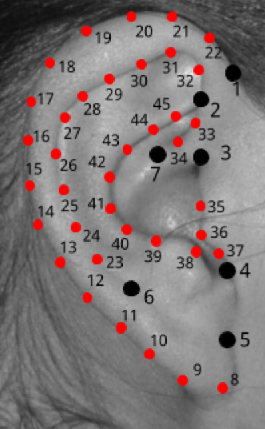
\includegraphics[scale=.4]{images/ear_landmarks}	\
	\caption{Landmarks on human ear in study of Cintas et al. \cite{cintas2016automatic}}
	\label{imgears}
\end{figure}
\fi
 
%In the past, landmarks on biological images are carried out manually or semi-automatically by applying some image processing techniques \cite{}. When the image processing techniques applied, segmentation is the most important step and this step becomes the bottleneck of the process. When the interested object easy to segment, the process may be provided the good results. But it could be a lack with the complex images (un-segmentable images). So, a method for landmarking without the help of segmentation step is very interested in and CNN has been chosen for this objective.

%As an association with the biologist, we study to develop an automatic method for predicting the landmarks on beetle's anatomical (Figs.\ref{figh1}, \ref{figt1}, \ref{fige1}, \ref{figlm1}, \ref{figrm1}). In the past, locating landmarks on biological images is mainly using image processing techniques where the object in the image is easily to segment. For example, in a previous work \cite{le2017maelab}, we have applied a series of algorithms to detect the landmarks automatically on beetles mandibles which are considered as the easied objects to segment (with an quality enough good for our need). In that work, the landmarks have been detected by registering two segmentations of images and then, using SIFT descriptor to refine the location of predicted landmarks. After the experiment, we have obtained good enough results on mandibles. Unfortunately, we have observed that the method did not provide good results when the segmentation is not precise, i.e. on pronotum or elytra images. This is explained why we have turned the automatically landmarking into another stage without any segmentation step. Using CNN for landmarking seems that a good choice for un-segmentable images.

\section{Overview of Convolutional Neural Network}
\label{sOverview}
CNN is a feedforward network which takes the information following one direction from the inputs to the outputs. Currently, CNNs have many different variations, i.e. AlexNet \cite{krizhevsky2012imagenet}, GoogLeNet \cite{szegedy2014going}, ResNet \cite{he2016deep}, but in general, it consists of convolutional and pooling layers which are stacked together to convolve and to down-sample the inputs. Then, they are followed by one or more fully connected layers to give the decision as the output of the network. 

Fig. \ref{imgcnn_network} shows an example of a CNN for classification problem. The network inputs directly an image to several stages of convolutional and pooling layers. Then, the representation is feed into three fully connected layers. A dropout layer is inserted after the second fully connected layer (it is repsented by some blue nodes). Finally, the last fully connected layer gives the category label for the input image. This architecture could be seen as the most popular one that we can find from the literature \cite{lecun1998gradient, krizhevsky2012imagenet}. However, several architectures have been proposed recurrently to improve the accuracy or to decrease the computation costs. In this section, we will mention to the most popular layers in a CNN: convolutional layers, pooling layers, and fully connected layers.

\begin{figure}[!h]
	\centering
	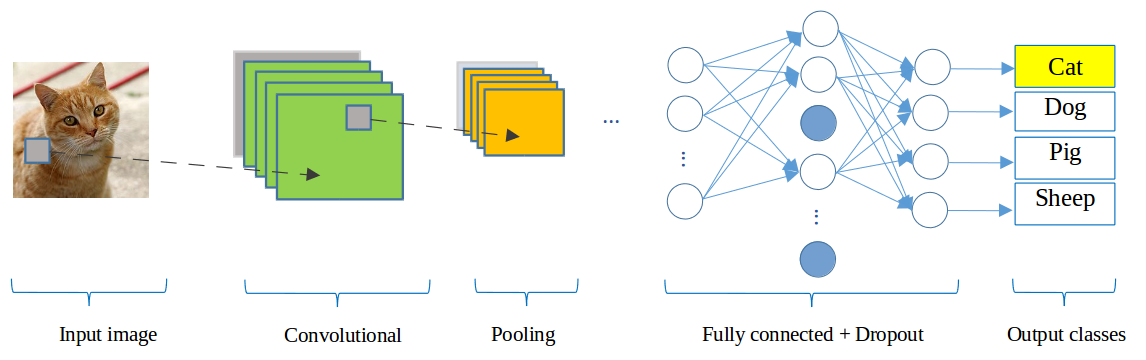
\includegraphics[scale=.3]{images/cnn_network_2}
	\caption{A CNN network for classification problem}
	\label{imgcnn_network}
\end{figure}

Convolutional (CONV) layers: use as a feature extractor by applying some learnable weights on the input images. The input image is convolved with the learnable weights in order to compute the new feature maps; then, the convolved results are sent through a nonlinear activation. In convolutional layer, the neurons are arranged into feature maps. All the neurons within a feature map have constrained to be equal; however, different features maps within the same convolutional layer have different weights so that several features can be extracted at each location of an input image. 

Pooling (POOL) layers : are mostly used to down-sampling the size of the input with the purpose to reduce the spatial resolution of the feature map to reduce the computation cost. Initially, it was common practice to use average pooling which propagates the average of all the input to the next layer. However, in more recent models \cite{krizhevsky2012imagenet, ciregan2012multi, li2015convolutional}, max pooling which propagates the maximum value (selecting the largest value) with a receptive field to the next layer. Fig. \ref{imgcnn_pooling} illustrates the differences between max and average pooling. Give an input image of size $4 \times 4$, if applying a $2 \times 2$ filter and stride of two is applied, the output will be had the size of $2 \times 2$ for both cases. However, the value in each element of the output is different because the max pooling outputs the maximum values of the filter region, while average pooling outputs the average value of the same region.

\begin{figure}[!h]
	\centering
	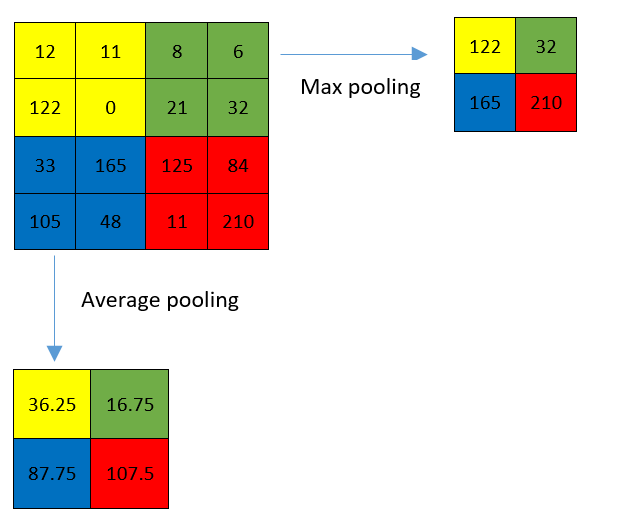
\includegraphics[scale=.5]{images/pooling}
	\caption{The results of different pooling}
	\label{imgcnn_pooling}
\end{figure}

Dropout (DROP) \cite{srivastava2014dropout} is a specific layer, it is used to prevent the over-fit of a neural network.
The term dropout mentions dropping the out units and their connections (incoming and outgoing)of a layer in the network. The units are dropped randomly with a probability $p$ independent with other units. The idea of dropout is not limited to feed-forward neural nets. Applying dropout technique will make the network become a collection of thinned networks because a number of units are dropped randomly at each presentation of training phase. So, training a neural network with dropout looks like training a collection of the thinned networks. Normally, the dropouts layers are placed after the fully connected layers, but it is possible to use dropout after the pooling layers with creating some kind of images noise augmentation.

Fully connected (FC) layers: are usually followed the convolutional and pooling layers which used to extract the abstract feature representations. A CNN may have one or more fully connected layers. It interprets the feature representations and performs a function of high-level reasoning (i.e. giving classification score) by applying the activation functions. In practice, the last fully connected layer refers to the output of the network and choosing the activation function is depended on which kind of problem that network solve, i.e. we usually softmax activation function for a classification problem but it is not useful in a support vector machine. 

To solve a problem by using deep learning, besides designing the network architecture then training dataset is also a very important thing. The success stories \cite{krizhevsky2012imagenet,he2016deep} have proved that CNN models work better with a large dataset. However, data in practice has usually not enough and we need to augment the data by applying some generation techniques (i.e. rotate, translate, flip the images). In the next section, we describe the procedure to augment our dataset, which has been considered as a small one.

\section{Data augmentation}
\label{Sdataaug}

The nature of deep learning algorithm is training the model on dataset repeatedly to reach the best accuracy. So, providing a large dataset will provide more learning cases for the model and it will clearly improve the learnable of the network. Unfortunately, we do not always have enough data for training in practice. One way to solve this problem is to create fake data from real data and to add it to the training set. Dataset augmentation has been a particularly effective technique for a specific problem. For example, the operations like translating, rotating or scaling the images have also effective in image classification problem. The fake images may be generated by translating (rotating or scaling) in each direction. Besides, injecting noise in the input can also see as a form of data augmentation. Our case is also not an exception, we work on a small dataset of beetles with $293$ images of beetles (for each anatomical part). This number is really modest to apply deep learning. So, an augmentation method has been described in this section to enlarge our dataset.

In our dataset, all the images are taken with the same camera in the same condition with a resolution of $(3264 \times 2448)$. Each image has a set of manual landmarks provided by biologists, i.e, each pronotum has $8$ landmarks, each head has $10$ landmarks (Fig. \ref{figbeetles}). Applying CNNs to train each part with a small number of images to reach good results is impossible. So, we need to augment the dataset before training the networks. Firstly, we have found that the original solution of the images $(3264 \times 2448)$ are heavy for the neural network. For performance considerations, in most of CNNs \cite{cintas2016automatic, lecun2010convolutional, sun2013deep}, the size of the input is limited to $(256 \times 256)$ pixels, so we have decided to down-sampling the images to a new resolution $(256 \times 192)$ (to respect the ratio between $x$ and $y$). Of course, the coordinates of manual landmarks have been also scaled to fit with the new resolution of the images. In the usual way, the transformations have been used to augment the dataset (i.e rotation, translation,\ldots) but the analysis of image by CNN is most often translation and rotation invariant. Therefore, two other procedures have been imaged to increase the number of images in the dataset $(256 \times 192)$.

\begin{figure}[htbp]
    \centering
\subfloat[Head]{\label{figh1}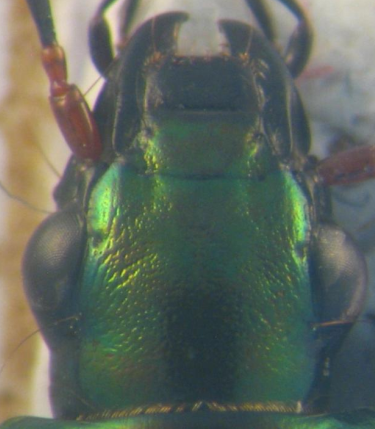
\includegraphics[width=0.2\textwidth]{images/orgHead}}~~    
    \subfloat[Pronotum]{\label{figh1}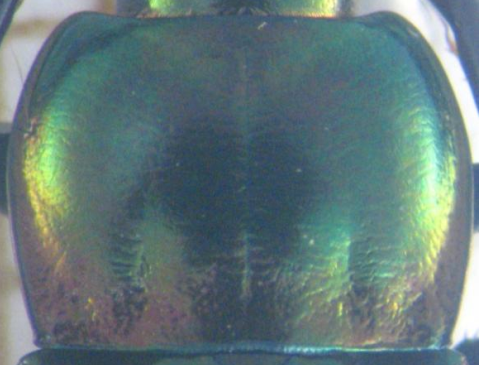
\includegraphics[width=0.2\textwidth]{images/orgThorax}}~~
\subfloat[Elytra]{\label{figh2}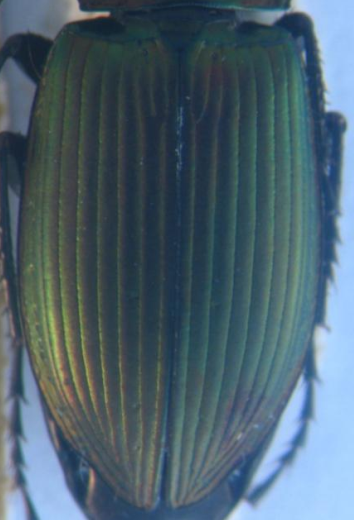
\includegraphics[width=0.16\textwidth]{images/orgElytra}} \\
	\subfloat[Head's manual landmarks]{\label{figh1}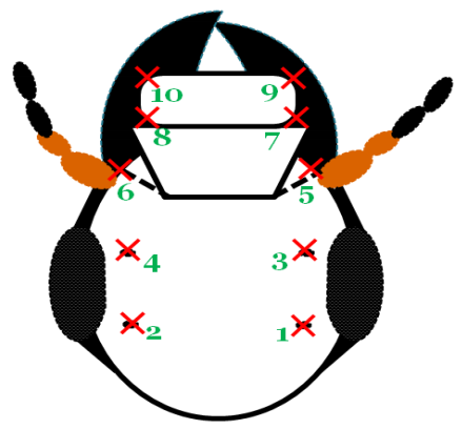
\includegraphics[width=0.2\textwidth]{images/lmHead}}~~	
	\subfloat[Pronotum's manual landmarks]{\label{figh1}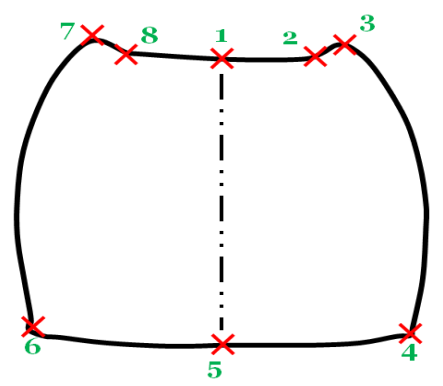
\includegraphics[width=0.2\textwidth]{images/lmThorax}}~~
\subfloat[Elytra's manual landmarks]{\label{figh2}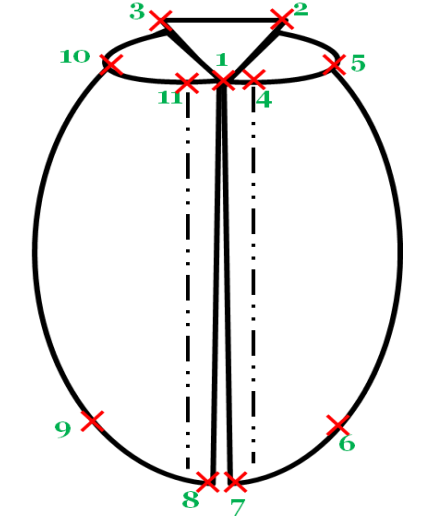
\includegraphics[width=0.16\textwidth]{images/lmElytra}} \\
	\subfloat[Left mandible]{\label{figh1}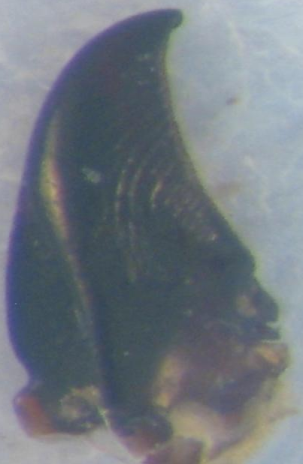
\includegraphics[width=0.13\textwidth]{images/orgLMandible}}~~
	\subfloat[Left mandible's manual landmarks]{\label{figh1}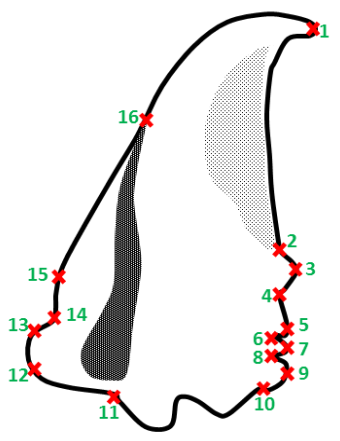
\includegraphics[width=0.15\textwidth]{images/lmLMandible}}~~	
	\subfloat[Right mandible]{\label{figh1}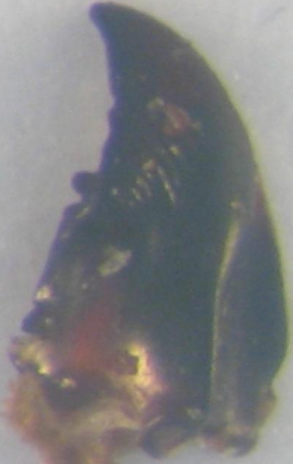
\includegraphics[width=0.13\textwidth]{images/orgRMandible}}~~
\subfloat[Right mandible's manual landmarks]{\label{figh2}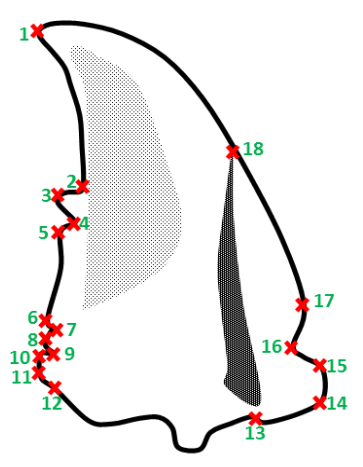
\includegraphics[width=0.15\textwidth]{images/lmRMandible}} \\
    \caption{The anatomicals of beetle and their manual landmarks}
    \label{figbeetles}
\end{figure}

The first procedure is to change the value of a color channel in the original image to generate a new image. According to that, a constant is added to one of the RGB channels each time it is used for training. Each constant is sampled in a uniform distribution $\in [1, N]$ to obtain a new value caped at $255$. For example, Fig. \ref{figaug1} shows an example when we added a constant $c = 10$ to each channel of an original image. Following this way, we can generate three version from an image.

\begin{figure}[h]
	\centering
	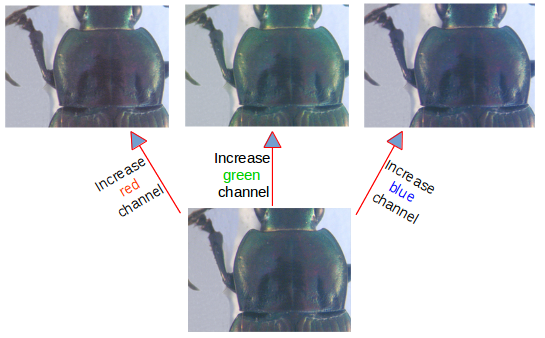
\includegraphics[scale=0.35]{images/inc_channels}
	\caption{A constant $c = 10$ has been added to each channel of an original image}
	\label{figaug1}
\end{figure}

In the second procedure, we have applied the opposite procedure to the first one. Instead of adding the value, we separate the channels of RGN into three gray-scale images as the network works on single channel images (Fig. \ref{figaug2}). At the end of the processes, we are able generate six versions from an original image. In total, we have $293 \times 7 = 2051$ images for each anatomical part of beetle (an original image and six generated images). However, we have not used all images for training and validation. So, we have chosen $260$ original images and their generations ($1820$ images) of each dataset for training and validation processes, the remaining images ($33$ original images) are used for test process.

\begin{figure}[h]
	\centering
	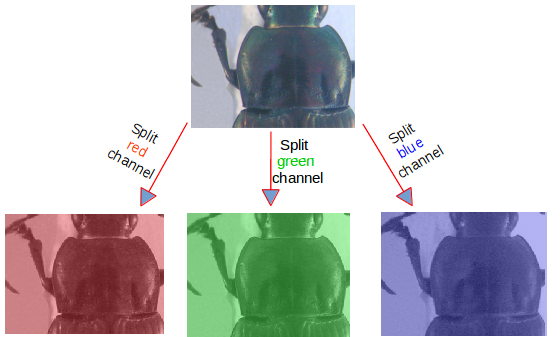
\includegraphics[scale=0.35]{images/sp_channels}
	\caption{Three channels (red, green, blue) are separated from original image}
	\label{figaug2}
\end{figure}

In practical, to obtain a fast convergence during the computing, it is useful to normalize the brightness of the images to $[0,1]$ instead of $[0, 255]$ and the coordinates of the landmarks have been also normalized \cite{lecun2012efficient}.

\section{Network architectures designing}
\label{Sneuralnetwork}
From the beginning of CNN, LeNet \cite{lecun1998gradient} can be considered as the first one, which has used to classify digits on hand-written numbers on cheques. The network is very simple by stack together the convolutional layers and max-pooling layers followed by full connected layers. Because of the limit of the resources at that time, this model is also constrained by the availability of computing. Until 2012, when computing resources are improved, AlexNet \cite{krizhevsky2012imagenet} was born and it has won the challenge by reducing the top-5 error in ImageNet challenge. AlexNet had a similar architecture as LeNet but it was deeper, bigger. Besides, the activation functions have been changed from Sigmoid \cite{han1995influence} to ReLU \cite{nair2010rectified} which have been proved more improvement in computing time. Additional, it had supplement the dropout layers to control overfitting. Based on the idea of the improvement, we have tried to design an architecture for landmarking on beetle images. This work is beginning with trying three network models before deciding the final architecture. Like other CNN models, we have employed the classical layers to construct the models, i.e., convolutional layers, maximum pooling layers, dropout layers and full-connected layers.

The first architecture is very classical one, it receives an image with the size of $(1 \times 192 \times 256)$ as the input. Then, the network consists of three repeated structures of a convolutional layer followed by a maximum pooling layer. Most of CNNs, the hyperparameters of convolutional layers have been set to increase the depth of the images from the first layer to the last layer. That is reflected in the setting of the number of filters at each convolutional layer. So, the depths of convolutional layers increase from $32, 64, $ and $128$ with different size of the kernels: $(3 \times 3)$, $(2 \times 2)$ and $(2 \times 2)$, respectively. Inserting pooling layers after a convolutional layers is a common periodcally. The pooling layer effects to progressively reduce the spatial size of the representation to reduce the number of parameters, computation in the network, and it also controls over-fitting. The operation of pooling layers is independent on every depth slice of the input. The most common form is a pooling layer with filters of size $(2 \times 2)$ and a stride of $2$. It downsamples every depth by $2$ along width and height of the input. Thefore, all the kernels of maximum pooling layers have the same size of $(2 \times 2)$ with a stride of $2$ as usual. At the end of the model, three full-connected layers have been added to extract the global relationship between the features and to procedure the outputs. The first of two full-connected layers are set to non-linearity to make sure these nodes interact well and take into account all possible dependencies at the feature level. The outputs of the full-connected layers are $500, 500$ and $16$. The output of the last full-connected layer corresponds to the coordinates ($x$ and $y$) of $8$ landmarks which we would like to predict. Fig. \ref{fignet1} shows details of the first model: The orange rectangles represent for convolutional layers while the yellow rectangles represent for maximum pooling layers and three full-connected layers with their parameters are presented at the end of the model.

\begin{figure}[!h]
	\centering
	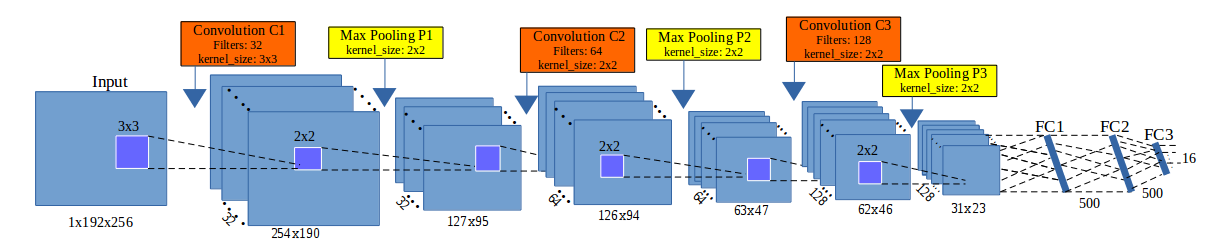
\includegraphics[scale=0.3]{images/net1}
	\caption{The architecture of the first model}
	\label{fignet1}
\end{figure}

The second architecture is modified from the first model. The layers are kept the same as the first one but the outputs of the first of two full-connected layers are changed from $500$ (in the first model) to $1000$ (Fig. \ref{fignet2}). Increasing the value at full-connected layers is hoping to obtain more features from convolutional layer and to prevent the over-fitting. 

\begin{figure}[h]
	\centering
	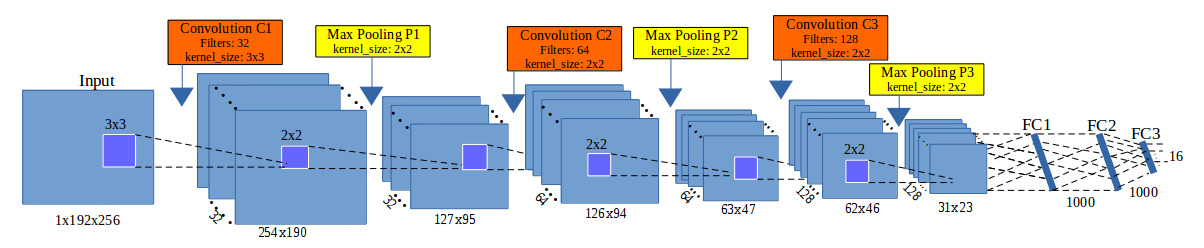
\includegraphics[scale=0.3]{images/net2}
	\caption{The architecture of the second model}
	\label{fignet2}
\end{figure}

To build the third architecture, we have used the definition of \textit{elementary block}. An {elementary block} is defined as a sequence of convolution ($C_{i}$), maximum pooling ($P_i$) and dropout ($D_i$) layers (Fig. \ref{figelementary}). This significantly reduces overfitting and gives major improvements over other regularization methods \cite{srivastava2014dropout}. The idea of dropout is to include some variations between different runs. During training phase, dropout samples are done from an exponential number of different ``thinned" network. At test phase, it is easy to approximate the effect of averaging the prediction of all thinned networks by simply using a single unthinned network with smaller weights. So, we have modified the architecture by combining some \textit{elementary blocks}. 

\begin{figure}[h]
	\centering
	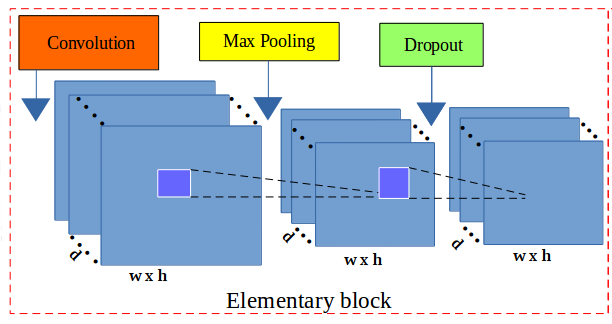
\includegraphics[scale=0.3]{images/elementary_block}
	\caption{The layers in an elementary block}
	\label{figelementary}
\end{figure}

Fig. \ref{fignet3} illustrates the layers in the third architecture. For our purpose, we have assembled \textbf{3 elementary blocks}. The parameters for each layer in each elementary block are as below, the list of values follows the order of elementary blocks ($i = [1..3]$):
\begin{itemize}
	\item CONV layers:
	\begin{itemize}
		\item Number of filters: $32, 64, $ and $128$
		\item Kernel filter sizes: $(3 \times 3), (2 \times 2), $ and $(2 \times 2)$
		\item Stride values: $1, 1, $ and $1$
		\item No padding is used for CONV layers 
	\end{itemize}
	\item POOL layers:
		\begin{itemize}
			\item Kernel filter sizes: $(2 \times 2), (2 \times 2), $ and $(2 \times 2)$
			\item Stride values: $2, 2, $ and $2$
			\item No padding is used for POOL layers
		\end{itemize}
	\item DROP layers:
		\begin{itemize}
			\item Probabilites: $0.1, 0.2, $ and $0.3$
		\end{itemize}
\end{itemize}

Three full-connected layers (FC) are kept the same as the second architecture: FC1 and FC2 have $1000$ outputs, the last full-connected layer (FC3) has $16$ outputs. As usual, a dropout layer is inserted between FC1 and FC2 with a probability equal to $0.5$.
\begin{figure}[h]
	\centering
	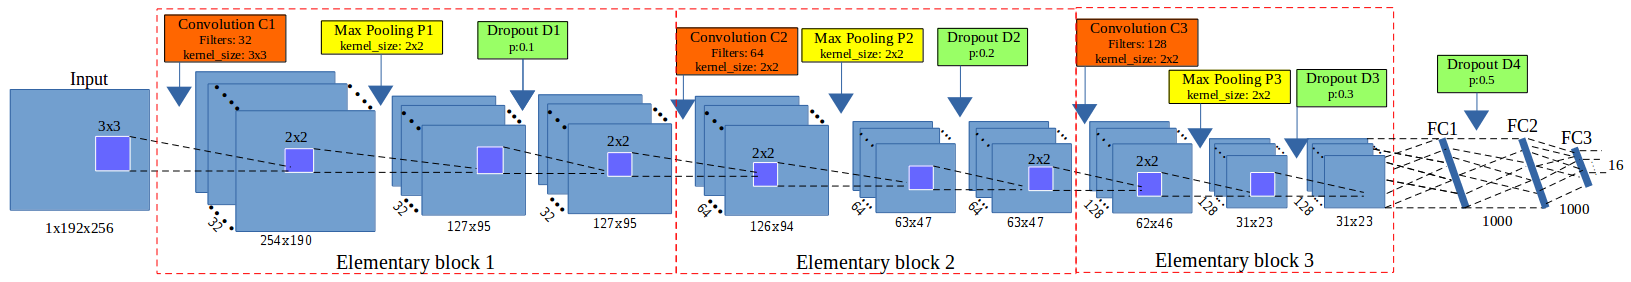
\includegraphics[scale=0.2]{images/arch_model}
	\caption{The architecture of the third model}
	\label{fignet3}
\end{figure}

The core of CNN is training over iteration. There are many ways to optimize the learning algorithm, but gradient descent \cite{lecun2012efficient} is currently a good choice to establish the way of optimizing the loss in neural network. The core idea is following the gradient until we statify with the results will remain the same. So, we have chosen gradient descent in the backward phase to update the values of learnable parameters and to increase the accuracy of the network. The networks are designed with a small sharing learning rate and a momentum. The learning rate is initialized at $0.03$ and stopped at $0.00001$, while the momentum is updated from $0.9$ to $0.9999$. Their values are updated over training time to fit with the number of epochs \footnote{An epoch is a single pass through the full training set}. The implementation of the architectures have been done on Lasagne framework \cite{lasagne} by Python. For more information about the model, you can see at our repository on GitHub: \texttt{https://github.com/linhlevandlu/CNN\_Beetles\_Landmarks}

\section{Experiments and results}
\label{sexperiments}
Before widely applying to all anatomical parts, we have firstly tried with pronotum part to evaluate the performance. The networks have been trained in $5, 000$ epochs on Ubuntu machine by using NVIDIA TITAN X cards. The set of images that used for training and validation are merged together. During the training, the images are chosen randomly from the dataset with a ratio of $60\%$ for training and $40\%$ for validation. The training step takes into account a pair of information (\textit{images, manual landmarks coordinates})  as training data. In the context of deep learning, landmark prediction can be seen as a regression problem. So, we have used Root Mean Square Error (RMSE) to compute the loss of implemented architectures. At the test phase, images without landmarks are given to the trained network to produce output coordinates of the predicted landmarks. The results then evaluated by comparing with the manual landmarks coordinates provided by biologists which have been seen as ground truth. 

Fig. \ref{figloss1} shows the training errors and the validation errors during traning phase of the first architecture. The blue curve presents the RMSE errors of training process while green curve is the validation errors. Clearly, over-fitting has appeared in the first model. The training losses are able to decrease but the validation losses are stable. In the second model (Section \ref{Sneuralnetwork}), we have modified the parameters of full-connected layers to prevent the over-fitting but it seems that this solution is still not suitable and the results are also the same with the first architecture.

\begin{figure}[!h]
	\centering
	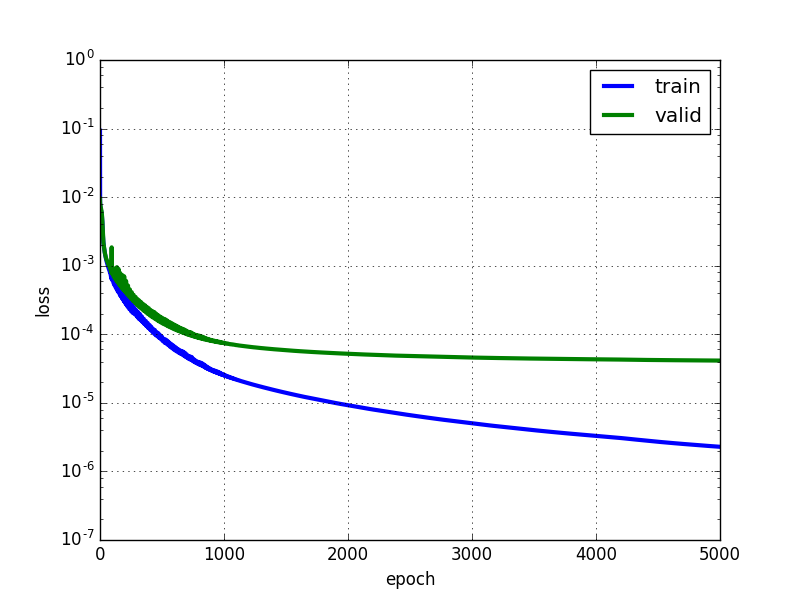
\includegraphics[scale=0.4]{images/cnnmodel3_5000_pronotum_v13_without_dropout_normalized_data_loss}
	\caption{The training and validation losses of the first model}
	\label{figloss1}
\end{figure}

Then, we have continued to train the third model on the same dataset of pronotum images. Fig. \ref{figloss2} illustrates the losses during the training of the third model. As the same meaning in Fig. \ref{figloss1}, the blue line is training loss, the green line is validation loss. In the opposite with two previous models, the losses are different (far) from the beginning but after several epochs, the loss values become more proximate and the over-fitting problem has been solved. This proves that adding dropout layers to build the elementary blocks have been effects to prevent over-fitting and contributory improve the accuracy of the model. \textit{So, we have decided to keep the architecture of the third model for our landmarking problem.}

\begin{figure}[!h]
	\centering
	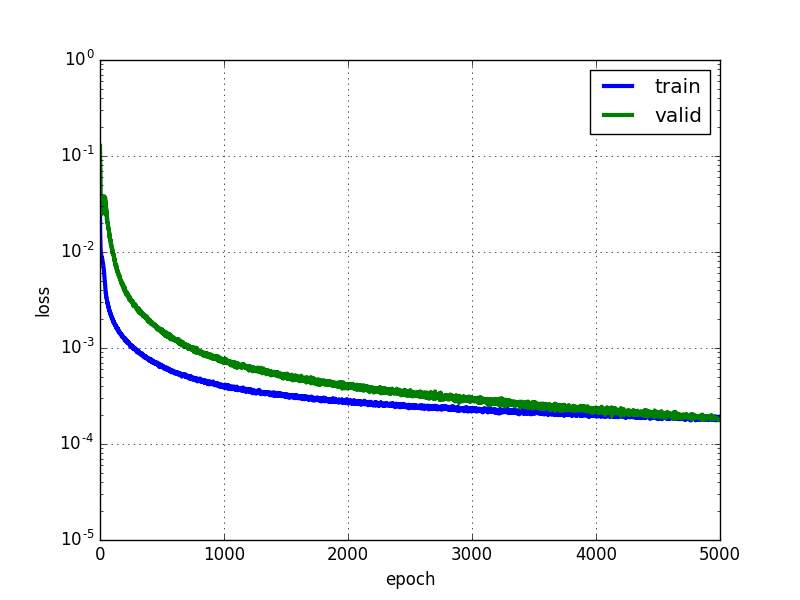
\includegraphics[scale=0.4]{images/loss_v16}
	\caption{The training and validation losses of the third model}
	\label{figloss2}
\end{figure}

In order to have the predicted landmarks for all pronotum images (instead of only $33$ images), we have applied \textit{cross-validation} to choose the test images, called \textit{round}. For each time, we have chosen a different fold of $33$ images as testing images, the remaining images are used as training and validation images ($293/33 \approx 9$ rounds). Following that, the network will be trained with different datasets, then the trained model will be used to predicted the lanmarks on the images in the corresponding test set. Table. \ref{tbltrainingloss} resumes the losses of $9$ rounds when we trained the third model on pronotum images. Clearly, the training loss/validation loss among rounds are not so large and the RMSE values are looking pretty good ($\approx 1.7 - 2.1$ pixels).

\begin{table}[h!]
	\centering
	\begin{tabular}{l l l}
	Round & Training loss & Validation loss \\ \hline
	1 & 0.00018 & 0.00019  \\ \hline
	2 & 0.00019 & 0.00021 \\ \hline
	3 & 0.00019 & 0.00026 \\ \hline
	4 & 0.00021 & 0.00029 \\ \hline
	5 & 0.00021 & 0.00029 \\ \hline
	6 & 0.00019 & 0.00018 \\ \hline
	7 & 0.00018 & 0.00018 \\ \hline
	8 & 0.00018 & 0.00021 \\ \hline
	9 & 0.00020 & 0.00027 \\ \hline
	\end{tabular}
	\caption{\small{The losses during training the third model on pronotum images}}
	\label{tbltrainingloss}
\end{table}

To evaluate the coordinates of predicted landmarks, the correlation metrics have been computed the correlation between the manual landmarks and their corresponding predicted one. Table. \ref{tblcorrelation} shows the correlation scores of $3$ metrics (using \textit{scikit-learn} \cite{pedregosa2011scikit}), i.e, coefficient of determination ($r^2$), explained variance (EV), and Pearson correlation. All of three metrics have the same possibility. The best score is $1.0$ if the correlation data is good, lower values are worse. It means that our predicted coordinates are very close with the ground truth. However, the measure is not enough good to provide a useful result to biologists. Moreover standing on the side of image processing, we are looking forward to  seeing the predicted coordinates than the statistical results.

\begin{table}[htbp]
	\centering
	\begin{tabular}{|c|p{2cm}|p{2cm}|p{2cm}|}
		Metric & $\mathbf{r^{2}}$ & \textbf{EV} & \textbf{Pearson} \\ \hline
		Score & $\textbf{0.9952}$ & $\textbf{0.9951}$ & $\textbf{0.9974}$ 
	\end{tabular}
	\caption{Correlation scores between manual landmarks and predicted landmarks}
	\label{tblcorrelation}
\end{table}

The main goal of computing is to predict the coordinates of landmarks, so the distances (in pixels) between the coordinates of manual landmarks and corresponding predicted landmarks have been taken into account on all images. Then, the average of distances are computed by landmarks. Table. \ref{tblavgpronotum} shows the average distances by landmarks on all images of pronotum dataset. With images of resolution $256 \times 192$, we can
consider that an error of $1\%$ corresponds to $2$ pixels that could
be an acceptable error. Unhappily, our results exhibit average
distance of $4$ pixels in the best case, landmark $1$ and more than
$5$ pixels, landmark $6$. Other error distances are more than $2\%$
pixels.

\begin{table}[htbp]
	\centering	
	\begin{tabular}{|c|c|}
		\hline
		\textbf{Landmark} & \textbf{Distance} (in pixels) \\ \hline
		1 & \textcolor{green}{\textbf{4.002}}  \\ \hline
		2 & 4.4831 \\ \hline
		3 & 4.2959 \\ \hline
		4 & 4.3865 \\ \hline
		5 & 4.2925 \\ \hline
		6 & \textcolor{red}{\textbf{5.3631}} \\ \hline
		7 & 4.636 \\ \hline
		8 & 4.9363 \\ \hline
	\end{tabular}
	\caption{The average distances on all images per landmark on pronotum images.}
	\label{tblavgpronotum}
\end{table}

Fig. \ref{figchartlm1} shows the distribution of the distances on the first landmark of all images. The accuracy based on the distance in each image can be
separated into three spaces: the images have the distance less
than average value ($4$ pixels): $56.66\%$; the images have the
distance from average value to $10$ pixels ($5\%$ acceptable errors): $40.27\%$; and the images have the distance
greater than $10$ pixels: $3.07\%$.

\begin{figure}[htbp]
	\centerline{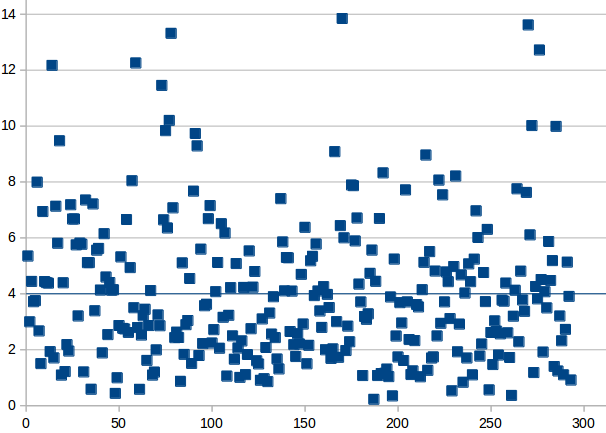
\includegraphics[scale=0.3]{images/statistic_pronotum_from_scratch_lm1}}
	\caption{The distribution of the distances on the first landmark. The blue line is the average value of all distances.}
	\label{figchartlm1}
\end{figure}

To illustrate this purpose, Fig. \ref{figrsexample} shows the predicted landmarks on two test images. One can note that even some predicted landmarks (Fig. \ref{figsub1}) are closed to the manual ones, in some case (Fig. \ref{figsub2}) the predicted ones are far from the expect results. This result explains why the average distance by landmarks are enough good while some predicted landmarks are so far from the manual one. So, the next step has been dedicated to the improvement of these results.

\begin{figure}[htbp]
    \centering
    \subfloat[Image with well-predicted landmarks]{\label{figsub1}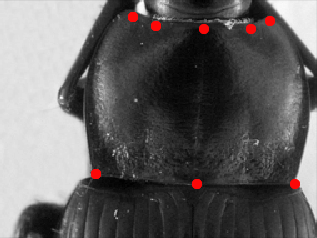
\includegraphics[width=0.35\textwidth]{images/fn_accuracy}}~~
\subfloat[Image with inaccuracy landmarks]{\label{figsub2}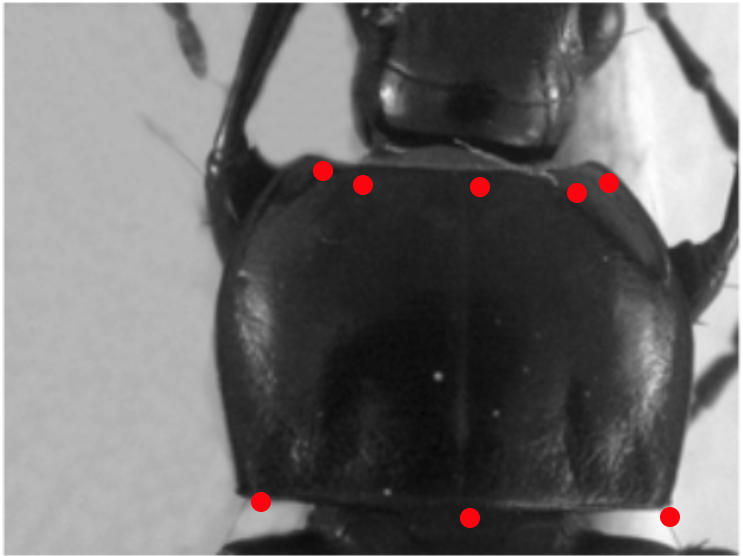
\includegraphics[width=0.35\textwidth]{images/plandmark2}}\\    
    \caption{The predicted landmarks, in red,  on the images in test set.}
    \label{figrsexample}
\end{figure}

From the success of the third architecture on pronotum dataset, we apply the same procedures (data augmentation, training,\ldots) on other parts of beetle: \textit{left mandible, right mandible, elytra, and head}. However, we have modified the number of output of the last full-connected layer to adapt with each dataset before training. According, the values at the last full-connected layer are set to $32$, $36$, $22$ and $20$ outputs corresponds to $16$, $18$, $11$ and $10$ landmarks on left mandible, right mandible, elytra and head, respectively. Of course, we have also applied cross-validation to select testing data to get all predicted landmarks for all images in each dataset. Then, the quality of predicted landmarks are evaluated by comparing with the corresponding manual landmarks (distance computation). Table. \ref{tblavg4parts} shows the average distances on each landmark of elytra, head, left and right mandibles anatomical, respectively. Comparing with the average distances on the pronotum part, the average distances on elytra and head parts are very close, but a little bit far on the mandible parts.

\begin{table}[htbp]
	\centering	
	\begin{tabular}{|c|c|c|c|c|}
		\hline
		\multirow{2}{*}{\textbf{Landmark}} & \multicolumn{4}{|c|}{\textbf{Distance (in pixels)}} \\ \cline{2-5}
		 & Right mandible & Left mandible & Elytra & Head  \\ \hline
		1 & \textcolor{red}{\textbf{9.4981}} & \textcolor{red}{\textbf{9.1267}} & \textcolor{green}{\textbf{3.8669}} & \textcolor{red}{\textbf{5.528}}  \\ \hline
2 & 7.1657 & \textcolor{green}{\textbf{6.7198}} & 3.973 & 5.1609  \\ \hline
3 & 7.242 & 6.8704 & 3.9166 & 5.3827 \\ \hline
4 & \textcolor{green}{\textbf{7.0436}} & 6.7719 & 3.8673 & 5.0345 \\ \hline
5 & 7.1599 & 7.125 & 4.0151 & 4.8393 \\ \hline
6 & 7.5699 & 6.9441 & 4.8426 & \textcolor{green}{\textbf{4.4516}} \\ \hline
7 & 7.4251 & 7.3158 & 5.2125 & 4.7937 \\ \hline
8 & 7.6636 & 7.4142 & \textcolor{red}{\textbf{5.4685}} & 4.5322 \\ \hline
9 & 7.7906 & 7.5846 & 5.2692 & 5.1412 \\ \hline
10 & 8.0197 & 7.6349 & 4.0709 & 5.0564 \\ \hline
11 & 8.314 & 7.6873 & 3.9896 & - \\ \hline
12 & 8.1564 & 8.4248 & - & - \\ \hline
13 & 8.8879 & 7.9983 & - & - \\ \hline
14 & 9.1842 & 7.4919 & - & - \\ \hline
15 & 8.7875 & 7.7903 & - & - \\ \hline
16 & 8.3141 & 8.5198 & - & - \\ \hline
17 & 8.2866 & - & - & - \\ \hline
18 & 8.8928 & - & - & - \\ \hline
	\end{tabular}
	\caption{The average distances on all images per landmark on right mandible, left mandible, elytra and head images.}
	\label{tblavg4parts}
\end{table}

\section{Resulting improvement by fine-tuning}
\label{sfineTuning}
The proposed network (third architecture) presented in Section \ref{Sneuralnetwork} have been trained from scratch on five datasets of beetles (left mandible, right mandible, pronotum, elytra, and head). At the first step, the network was able to predict the landmarks on the images. But as we have discussed, even if the strength of the correlation seems to validate the results, when we display the predicted landmarks on the images, the quality of the predicted coordinates are also not enough precise, and the average error are also still high (of course, we have the distances are higher than the average distances).

In order to reach more acceptable results for biologists, we have broadened model with another step of deep learning: \textbf{transfer learning}. That is a method enables to re-uses the model developed for a specific task/dataset to lead another task (called \textit{target task}) with another dataset. This process allows rapid process and improves the performance of the model on the target task \cite{torrey2009transfer}. The most popular example has been given with the project ImageNet of Google \cite{imagenet_cvpr09} which has labeled several millions of images. The obtained parameter values which can be used in another context to classify another dataset, eventually very different dataset \cite{margeta_mri}. The name of this procedure to re-use parameters to pretrain a model is currently called \textbf{fine-tuning}.

Fine-tuning does not only replace and retrain the model on
the new dataset but also fine-tunes the weights of a trained
model by continuing the backpropagation. Unfortunately,
some rapid tests have shown that re-using ImageNet features
has not been relevant for our application. We have designed a
way to reproduce the method with our own data. It is worth
noting that of course the size of data to pre-train has drastically decreased. For our pre-training step, the network has been
trained on the whole dataset including the images of three parts
of beetle \textit{i.e pronotum, elytra and head}. Then, the trained model
has been used to fine-tune and test on each dataset.
\subsection{Data preparation and training}
The images training dataset is combined from the images of three sets: \textit{pronotum, elytra, and head} (after augmentation). When applying the training from the scratch, we have used cross-validation to select the data ($9$ folds). It means that for each dataset, we have some different training data and corresponding testing data. So, the images that use to train the model are just select from one of the folds in each dataset. Specifically, we have taken $1, 820$ images of each part. In total, it includes $5, 460$ images $(260 \times 7 \times 3)$. 

\begin{figure}[htbp]
	\centerline{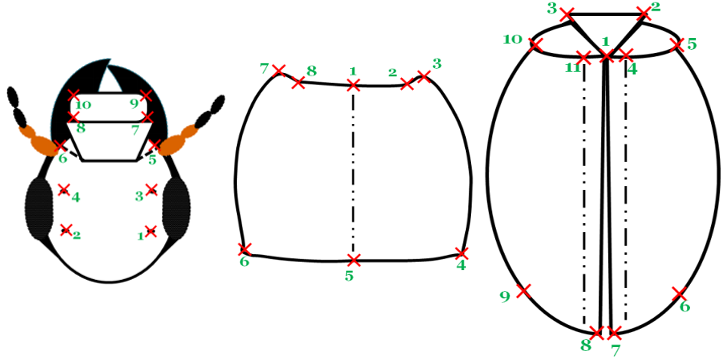
\includegraphics[scale=0.5]{images/merge}}
	\caption{A presentation of head, pronotum and elytra part with
corresponding manual landmarks}
	\label{figmerge}
\end{figure}

However, another problem has been appeared when we combined the images from different dataset. That is the different number of landmarks on each part: \textit{$8$ landmarks on pronotum part, $10$ landmarks on head part, and $11$ landmarks on elytra part}. Fig. \ref{figmerge} shows the possition of the landmarks on each part. Because of the meaning of landmarks on each anatomical part for biologists, we cannot insert the landmarks arbitrary. So,  we have decided to keep the landmarks on pronotum as reference and to remove the landmarks on elytra and head parts instead of adding. We kept $8$ (landmarks) as a reference number, then we have removed the supernumerary when it is unnecessary. Specifically, we have removed three landmarks on the elytra part ($1^{st}, 6^{th}, 9^{th}$), and two landmarks on the head part ($5^{th}, 6^{th}$). 

During training the proposed architecture on the combined dataset, the parameters of the network (learning rate, momentum, \ldots) are kept the same as training from scratch but the number of epochs are increased to $10, 000$ instead of $5, 000$ to achieve better learning on the parameters (weights). Additional, we have shuffled the training data because the neural network learns the faster from the most unexpected sample. It is advisable to choose a sample at each iteration that is the most unfamiliar to the system. Shuffling the examples will be helped the model works with different anatomical parts rather than the same anatomical samples in each training time.

\subsection{Fine-tuning on each dataset}
The combined dataset then used to train the third architecture with $16$ outputs ($8$ landmarks). Then, the trained model is used to fine-tuning on each dataset. To compare the result with the previous one, we have also fine-tuned the trained model with different dataset by applying cross-validation. Firstly, we consider on the losses during fine-tuning. \textit{For example}, Table. \ref{tblftpronotum}, \ref{tblftbody}, \ref{tblfthead} show the losses during fine-tuning on pronotum, elytra, and head dataset, respectively. Comparing with the losses when we trained the model from scratch, \textit{i.e.} on pronotum, the validation losses of all round in this scenario have been significantly decreased (around $40\%$).

On each part, the landmarks are predicted on the test images. Then, the average error based on the distances between predicted and corresponding manual landmarks have been also computed. Tables. \ref{tblcmppronotum}, \ref{tblcmpbody}, \ref{tblcmphead}, \ref{tblcmpmg}, and \ref{tblcmpmd} show the average distances per landmark on pronotum, elytra, head, left and right mandibles dataset, respectively. \textbf{From scratch} columns remind the previously average distances. \textbf{Fine-tune} columns present the new average distances after applying fine-tuning on each part. It is clearly shown that the result of predicted landmarks with the help of fine-tuning is more precise than training from scratch. For example, the average distance at each landmark has decreased. Additional, when comparing the average distances between two processes, the worse case of fine-tuning process is still better than the best case of training from scratch.

\begin{table}[htbp]
	\begin{minipage}[t]{0.45\textwidth}
	\centering
	\begin{tabular}{l p{1.5cm} p{1.5cm}}
	Round & Training loss & Validation loss \\ \hline
	1 & 0.00019 & 0.00009  \\ \hline
	2 & 0.00018 & 0.00010 \\ \hline
	3 & 0.00018 & 0.00010 \\ \hline
	4 & 0.00019 & 0.00008 \\ \hline
	5 & 0.00019 & 0.00009 \\ \hline
	6 & 0.00018 & 0.00008 \\ \hline
	7 & 0.00019 & 0.00008 \\ \hline
	8 & 0.00018 & 0.00006 \\ \hline
	9 & 0.00018 & 0.00009 \\ \hline
	\end{tabular}
	\caption{The losses during fine-tuning model on pronotum dataset}
	\label{tblftpronotum}
\end{minipage}
\hfill
\begin{minipage}[t]{0.45\textwidth}
\centering
\begin{tabular}{|c|c|c|}
\hline
\textbf{$\#$LM} & \textbf{From scratch} & \textbf{Fine-tune} \\ \hline
1 & \textcolor{green}{\textbf{4.00 }}& \textcolor{green}{\textbf{2.49}}  \\ \hline
2 & 4.48 & 2.72  \\ \hline
3 & 4.30  & 2.65 \\ \hline
4 & 4.39  & 2.77 \\ \hline
5 & 4.29  & \textcolor{green}{\textbf{2.49}} \\ \hline
6 & \textcolor{red}{\textbf{5.36}}  & \textcolor{red}{\textbf{3.05}} \\ \hline
7 & 4.64  & 2.68 \\ \hline
8 & 4.94  & 2.87 \\ \hline
\end{tabular}
\caption{The average error distances per landmark of two deep learning processes on pronotum images}
\label{tblcmppronotum}
\end{minipage}
\end{table}

\begin{table}[htbp]
	\begin{minipage}[t]{0.45\textwidth}
	\centering
	\begin{tabular}{c p{1.5cm} p{1.5cm}}
	Round & Training loss & Validation loss \\ \hline
	1 & 0.00020 & 0.00006  \\ \hline
	2 & 0.00020 & 0.00006 \\ \hline
	3 & 0.00021 & 0.00006 \\ \hline
	4 & 0.00021 & 0.00006 \\ \hline
	5 & 0.00019 & 0.00006 \\ \hline
	6 & 0.00019 & 0.00006 \\ \hline
	7 & 0.00018 & 0.00005 \\ \hline
	8 & 0.00020 & 0.00006 \\ \hline
	9 & 0.00019 & 0.00006 \\ \hline
	\end{tabular}
	\caption{The losses during fine-tuning model on elytra dataset}
	\label{tblftbody}
\end{minipage}
\hfill
\begin{minipage}[t]{0.45\textwidth}
\centering
\begin{tabular}{|c|c|c|}
\hline
\textbf{$\#$LM} & \textbf{From scratch} & \textbf{Fine-tune} \\ \hline
1 & \textcolor{green}{\textbf{3.87}} & 2.34  \\ \hline
2 & 3.97 & 2.27  \\ \hline
3 & 3.92  & 2.27 \\ \hline
4 & \textcolor{green}{\textbf{3.87}}  & \textcolor{green}{\textbf{2.25}} \\ \hline
5 & 4.02  & 2.27 \\ \hline
6 & 4.84  & 3.14 \\ \hline
7 & 5.21  & 3.14 \\ \hline
8 & \textcolor{red}{\textbf{5.47}}  & 3.29 \\ \hline
9 & 5.27  & \textcolor{red}{\textbf{3.42}} \\ \hline
10 & 4.07  & 2.49 \\ \hline
11 & 3.99  & 2.30 \\ \hline
\end{tabular}
\caption{The average error distances per landmark of two deep learning processes on elytra images}
\label{tblcmpbody}
\end{minipage}
\end{table}

\begin{table}[htbp]
\begin{minipage}[t]{0.45\textwidth}
	\centering
	\begin{tabular}{l p{1.5cm} p{1.5cm}}
	Round & Training loss & Validation loss \\ \hline
	1 & 0.00022 & 0.00007  \\ \hline
	2 & 0.00022 & 0.00007 \\ \hline
	3 & 0.00023 & 0.00008 \\ \hline
	4 & 0.00023 & 0.00008 \\ \hline
	5 & 0.00022 & 0.00008 \\ \hline
	6 & 0.00023 & 0.00007 \\ \hline
	7 & 0.00022 & 0.00008 \\ \hline
	8 & 0.00023 & 0.00007 \\ \hline
	9 & 0.00024 & 0.00008 \\ \hline
	\end{tabular}
	\caption{The losses during fine-tuning model on head dataset}
	\label{tblfthead}
\end{minipage}
\hfill
\begin{minipage}[t]{0.45\textwidth}
\centering
\begin{tabular}{|c|c|c|}
\hline
\textbf{$\#$LM} & \textbf{From scratch} & \textbf{Fine-tune} \\ \hline
1 & \textcolor{red}{\textbf{5.53}} & \textcolor{red}{\textbf{3.03}}  \\ \hline
2 & 5.16 & 2.94  \\ \hline
3 & 5.38  & 2.96 \\ \hline
4 & 5.03  & 2.88 \\ \hline
5 & 4.84  & 2.76 \\ \hline
6 & \textcolor{green}{\textbf{4.45}}  & 2.67 \\ \hline
7 & 4.79  & 2.29 \\ \hline
8 & 4.53  & \textcolor{green}{\textbf{2.20}} \\ \hline
9 & 5.14  & 2.57 \\ \hline
10 & 5.06  & 2.44 \\ \hline
\end{tabular}
\caption{The average error distances per landmark of two deep learning processes on head images}
\label{tblcmphead}
\end{minipage}
\end{table}

\begin{table}[htbp]
\begin{minipage}[t]{0.45\textwidth}
\centering
\begin{tabular}{|c|c|c|}
		\hline
		\textbf{$\#$LM} & \textbf{From scratch} & \textbf{Fine-tune} \\ \hline
		1 & \textcolor{red}{\textbf{9.1267}} & \textcolor{red}{\textbf{6.7655}} \\ \hline
		2 & \textcolor{green}{\textbf{6.7198}} & \textcolor{green}{\textbf{5.2952}} \\ \hline
		3 & 6.8704 & 5.3468 \\ \hline
		4 & 6.7719 & 5.332 \\ \hline
		5 & 7.125 & 5.4391 \\ \hline
		6 & 6.9441 & 5.3004 \\ \hline
		7 & 7.3158 & 5.5314 \\ \hline
		8 & 7.4142 & 5.6486 \\ \hline
		9 & 7.5846 & 5.8864 \\ \hline
		10 & 7.6349 & 5.9245 \\ \hline
		11 & 7.6873 & 5.972 \\ \hline
		12 & 8.4248 & 6.5755 \\ \hline
		13 & 7.9983 & 6.1067 \\ \hline
		14 & 7.4919 & 5.6307 \\ \hline
		15 & 7.7903 & 5.8522 \\ \hline
		16 & 8.5198 & 7.174 \\ \hline
	\end{tabular}
\caption{The average error distances per landmark of two deep learning processes on left mandible images}
\label{tblcmpmg}
\end{minipage}
\hfill
\begin{minipage}[t]{0.45\textwidth}
\centering
\begin{tabular}{|c|c|c|}
\hline
\textbf{$\#$LM} & \textbf{From scratch} & \textbf{Fine-tune} \\ \hline
		1 & \textcolor{red}{\textbf{9.4981}} & 6.3236 \\ \hline
	2 & 7.1657 & 5.1347 \\ \hline
	3 & 7.242 & 5.1613 \\ \hline
	4 & \textcolor{green}{\textbf{7.0436}} & \textcolor{green}{\textbf{5.0537}} \\ \hline
	5 & 7.1599 & 5.1372 \\ \hline
	6 & 7.5699 & 5.301 \\ \hline
	7 & 7.4251 & 5.2064 \\ \hline
	8 & 7.6636 & 5.5168 \\ \hline
	9 & 7.7906 & 5.6858 \\ \hline
	10 & 8.0197 & 5.7495 \\ \hline
	11 & 8.314 & 6.1975 \\ \hline
	12 & 8.1564 & 6.1898 \\ \hline
	13 & 8.8879 & 6.7612 \\ \hline
	14 & 9.1842 & \textcolor{red}{\textbf{7.0694}} \\ \hline
	15 & 8.7875 & 6.5293 \\ \hline
	16 & 8.3141 & 6.1147 \\ \hline
	17 & 8.2866 & 6.2881 \\ \hline
	18 & 8.8928 & 6.8367 \\ \hline
\end{tabular}
\caption{The average error distances per landmark of two deep learning processes on right mandible images}
\label{tblcmpmd}
\end{minipage}
\end{table}

In another view, Fig. \ref{figdist5parts} shows the comparison of the average distance distributions on each dataset in two procedures (from scratch and fine-tuning). In which:
\begin{itemize}
	\item \textbf{Blue} curves: present for the average distances on each landmarks when we train the model from scratch.
	\item \textbf{Orange} curves: describe for the average distance on each landmark when we fine-tune the trained model.
	\item \textbf{Black} curves (in the case of left and right mandibles): illuslate for the average distances when we applied the image processing procedures to predict the landmarks on segmentable images.
\end{itemize}

\iffalse
\begin{figure}[htbp]
	\centerline{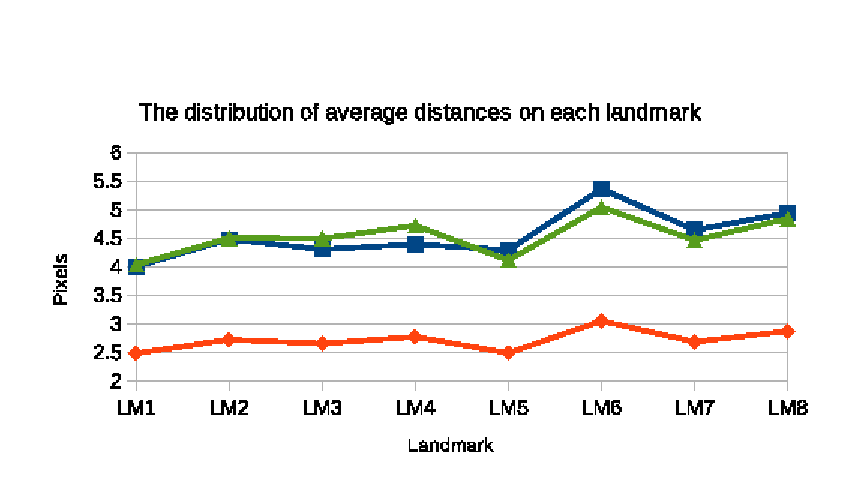
\includegraphics[scale=0.55]{images/prono_part}}
	\caption{The distribution of average distances on each landmark of pronotum part.}
	\label{figdistpronotum}
\end{figure}

\begin{figure}[htbp]
	\centerline{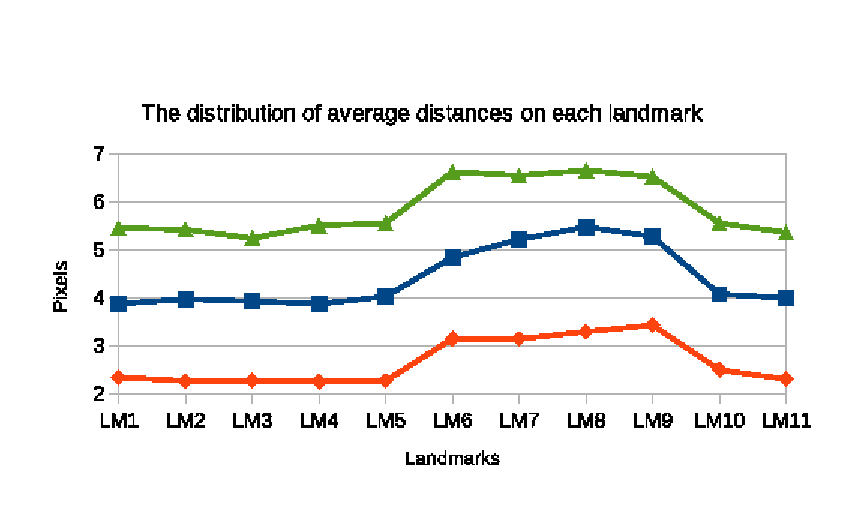
\includegraphics[scale=0.55]{images/body_part}}
	\caption{The distribution of average distances on each landmark of elytra part.}
	\label{figdistelytra}
\end{figure}

\begin{figure}[htbp]
	\centerline{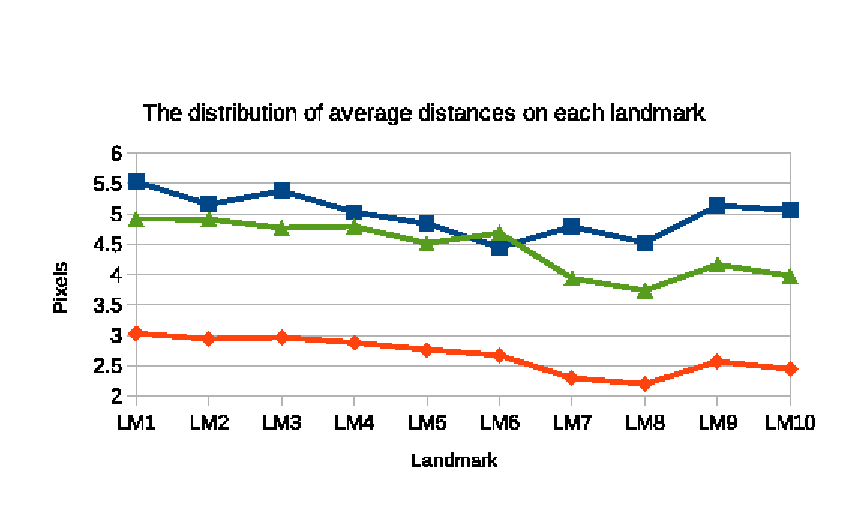
\includegraphics[scale=0.55]{images/head_part}}
	\caption{The distribution of average distances on each landmark of head part.}
	\label{figdisthead}
\end{figure}
\fi
\begin{figure}[htbp]
    \centering
    \subfloat[Left mandible]{\label{}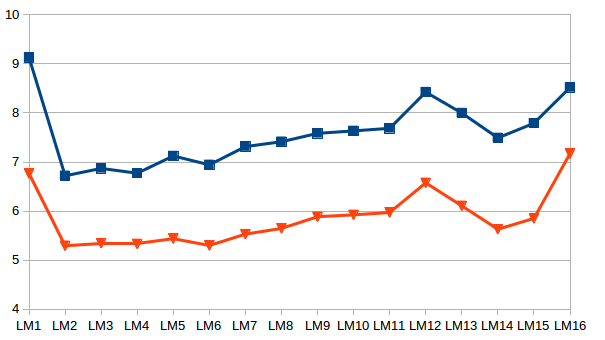
\includegraphics[width=0.5\textwidth]{images/mg_part}}~~
	\subfloat[Right mandible]{\label{}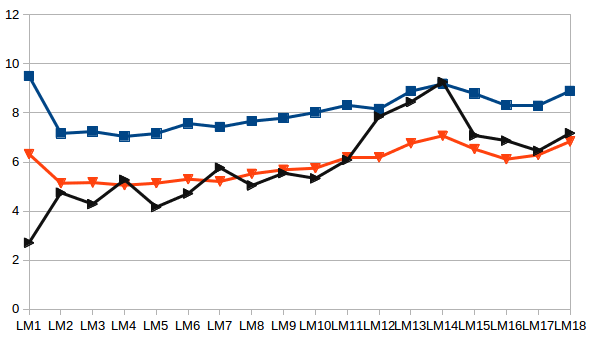
\includegraphics[width=0.5\textwidth]{images/md_part}}\\
    \subfloat[Head]{\label{}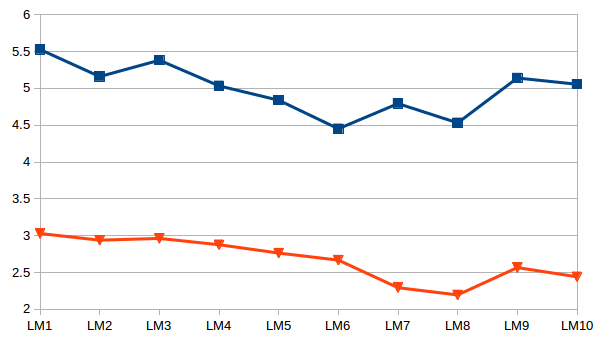
\includegraphics[width=0.5\textwidth]{images/tete_part}}~~
	\subfloat[Elytra]{\label{}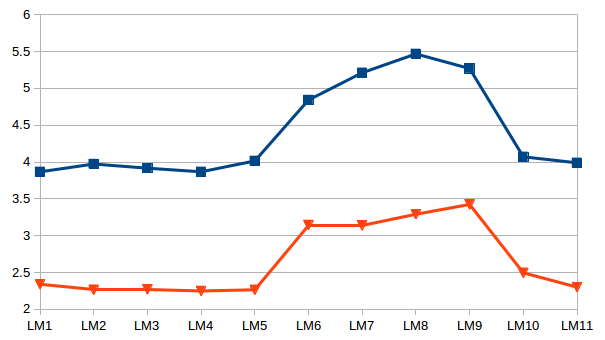
\includegraphics[width=0.5\textwidth]{images/elytre_part}}\\
	\subfloat[pronotum]{\label{}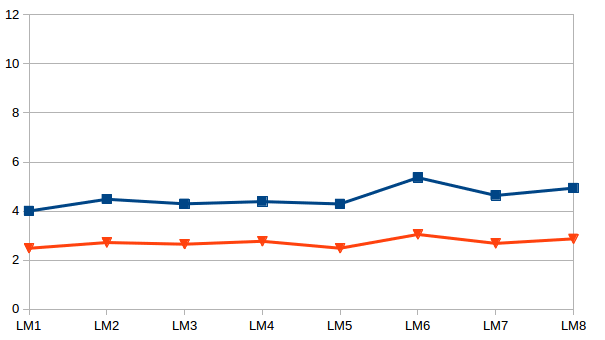
\includegraphics[width=0.5\textwidth]{images/pronotum_part.png}}
    \caption{The distribution of average distances on each landmark of each beetle's anatomical. Black, blue, and orange lines present for the results of image processing procedures, deep learning (from scratch and fine-tuning), respectively. }
    \label{figdist5parts}
\end{figure}

The fine-tuning process has improved the results of the proposed architecture on both $5$ datasets: left, right mandible, pronotum, elytra and head. All the average distances are significantly decreased. Specially, the results have been improved $\approx 26.9\%$ on left mandible, $\approx 22.8\%$ on right mandible, $\approx 40.3\%$ on pronotum, $\approx 39.8\%$ on elytra, and $\approx 46.4\%$  on head part based on considering the average distances per landmark. Addition, in the cases of pronotum and head part, even if we plus the average distance and its standard deviation, the results are also less than the result when we trained the model from scratch. For segmentable images, we have a comparison between the results of deep learning and early method where we have applied image processing techniques to predict the landmarks \cite{le2017maelab}. Clearly, the result with fine-tuning has improved the location of estimated landmarks. Even the average distances which obtained from scratch training are still high but they are more stable than the results from the early method: most of the average distance(or landmarks) of left mandibles are less than the results of the early method, while the average distances are very closed in the case of right mandibles.

%\pagebreak
To compare the results between image processing procedures and deep learning, we have run the test on an image of all parts in both methods. Then, we have calculated the distances between manual and predicted landmarks (in both cases). Fig. \ref{figmn5parts} shows the locations of manual and predicted landmarks on each beetle's part from both two methods. In these images, the \textbf{red points} present the manual landmarks, the \textbf{yellow points} are estimated landmarks from image processing procedures and the \textbf{green points} are predicted landmarks which have been provided by deep learning.

\begin{figure}[htbp]
    \centering
    \subfloat[Left mandible]{\label{}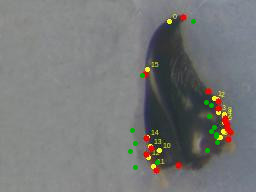
\includegraphics[width=0.5\textwidth]{images/mg_3c}}~~
	\subfloat[Right mandible]{\label{}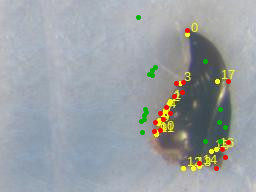
\includegraphics[width=0.5\textwidth]{images/md_3c}}\\
    \subfloat[Head]{\label{}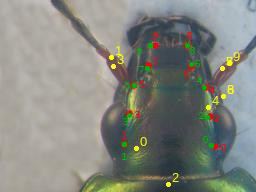
\includegraphics[width=0.5\textwidth]{images/tete_3c}}~~
	\subfloat[Elytra]{\label{}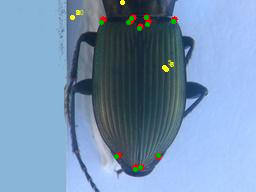
\includegraphics[width=0.5\textwidth]{images/elytre_3c}}\\
	\subfloat[Pronotum]{\label{}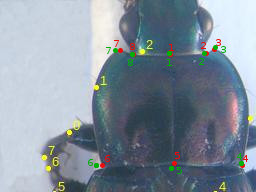
\includegraphics[width=0.5\textwidth]{images/pronotum_3c}}
    \caption{The presentation of manual and predicted landmarks on each beetle's part by applying two methods: image processing procedures and deep learning. The red points, yellow points, and green points present for manual landmarks, estimated landmarks by applying image processing procedures and using deep learning, respectively. }
    \label{figmn5parts}
\end{figure}

Fig. \ref{fig0015parts} shows the distances by landmarks when we did a test on one image of each part. In these charts, the \textbf{black lines} present the distances when we apply the calculation on image processing procedures; the \textbf{blue and orange lines} show the distances with deep learning: training from scratch and fine tuning, respectively. As described in \cite{le2017maelab}, we have combined some image processing procedures to output the predicted landmarks and this has become also a disadvantage of this method. If one procedure of them provides a bad result, it will affect the final result, i.e. if the result of segmentation step is bad, it seems that can not provide the output. In all beetle's anatomical, the mandibles are considered as the easy case to segment because the images are clear (they just contains the mandibles); while other parts are much noise, besides the main objects they have also the subcomponents of beetle, i.e. leg, antennae, \ldots. That explains why we have obtained good results on mandibles but bad results on head, elytra, and pronotum part when applying the image processing procedures. In the opposite side, the results with deep learning, either training from scratch or fine-tuning, are very stable (Fig. \ref{fig0015parts}). In the case of mandibles, which have good results from image processing techniques, then the results from deep learning are not much difference.

\begin{figure}[htbp]
    \centering
    \subfloat[Left mandible]{\label{}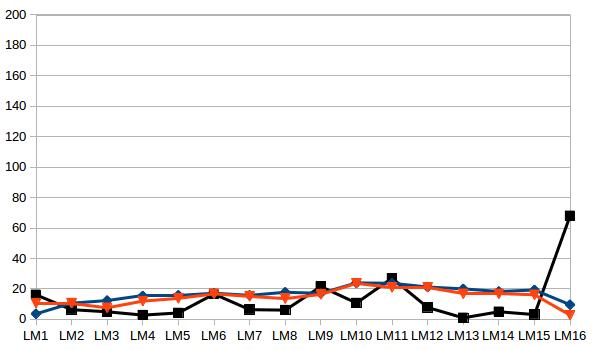
\includegraphics[width=0.5\textwidth]{images/mg001_2}}~~
	\subfloat[Right mandible]{\label{}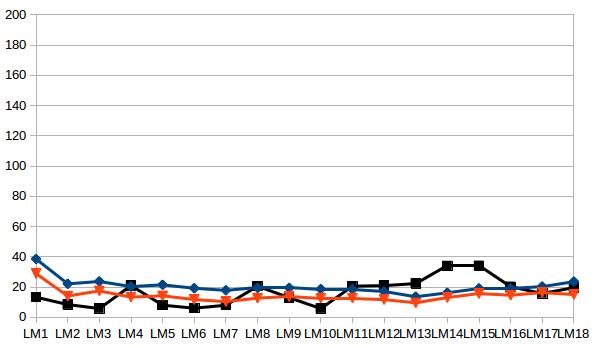
\includegraphics[width=0.5\textwidth]{images/md001_2}}\\
    \subfloat[Head]{\label{}\includegraphics[width=0.5\textwidth]{images/tete001_2}}~~
	\subfloat[Elytra]{\label{}\includegraphics[width=0.5\textwidth]{images/elytre001_2}}\\
	\subfloat[Pronotum]{\label{}\includegraphics[width=0.5\textwidth]{images/pronotum001_2}}
    \caption{The distances between manual and predicted landmarks of a test image when applying different techniques of each beetle's anatomical. Black, blue, and orange lines present for the results of image processing procedures, deep learning (from scratch and fine-tuning), respectively. }
    \label{fig0015parts}
\end{figure}

\pagebreak
\section{Conclusion}
\label{sconclusion}
In this work, we have presented how to apply convolutional neural network to predict the landmark on 2D anatomical images of beetles. After going through many trial models, we have presented a convolutional neural network for automatic detection landmarks on anatomical images of beetles which includes the repeated of some elementary blocks (an elementary block consists of a convolutional layer, a max pooling layer, and a dropout layer) followed by fully connected layers. Then, the proposed model have been trained and tested by using two strategies: \textit{train from scratch} and \textit{fine-tuning}. 

In our case, the size of dataset is limited. Therefore, we have applied the image processing techniques to augment dataset. The predicted landmarks have been evaluated by calculating the distance between manual landmarks and corresponding predicted landmarks. Then, the average of distance errors on each landmarks has been considered.

The results have been shown that using the convolutional network to predict the landmarks on biological images leads to satisfying results without need for segmentation step on the object of interest. The
best set of estimated landmarks has been obtained after a step
of fine-tuning using the whole set of images that we have for the
project, i.e. about all beetle parts. The quality of prediction allows using automatic landmarking to replace the manual ones.
\section*{References}

\bibliography{includes/mybibfile}

\end{document}




\begin{table}[htbp]
\begin{minipage}{0.5\linewidth}
	\centering
	\begin{tabular}{|c|c|}
		\hline
		\textbf{Landmark} & \textbf{Distance} (in pixels) \\ \hline
		1 & 3.8669  \\ \hline
		2 & 3.9730 \\ \hline
		3 & 3.9166 \\ \hline
		4 & 3.8673 \\ \hline
		5 & 4.0151 \\ \hline
		6 & 4.8426 \\ \hline
		7 & 5.2125 \\ \hline
		8 & 5.4685 \\ \hline
		9 & 5.2692 \\ \hline
		10 & 4.0709 \\ \hline
		11 & 3.9896 \\ \hline
	\end{tabular}
	\caption{\small{The average distance on all images per landmark on \textbf{elytra} images}}
	\label{tblavgdiselytra}
\end{minipage}
\hfill
\begin{minipage}{0.5\linewidth}
	\centering
	\begin{tabular}{|c|c|}
		\hline
		\textbf{Landmark} & \textbf{Distance} (in pixels) \\ \hline
		1 & 5.5280  \\ \hline
		2 & 5.1609 \\ \hline
		3 & 5.3827 \\ \hline
		4 & 5.0345 \\ \hline
		5 & 4.8393 \\ \hline
		6 & 4.4516 \\ \hline
		7 & 4.7937 \\ \hline
		8 & 4.5322 \\ \hline
		9 & 5.1412 \\ \hline
		10 & 5.0564 \\ \hline
	\end{tabular}
	\caption{\small{The average distance on all images per landmark on \textbf{head} images}}
	\label{tblavgdishead}
\end{minipage}
\end{table}

\begin{table}[htbp]
\begin{minipage}{0.5\linewidth}
	\centering
	\begin{tabular}{|c|c|}
		\hline
		\textbf{Landmark} & \textbf{Distance} (in pixels) \\ \hline
		1 & 9.1267  \\ \hline
		2 & 6.7198 \\ \hline
		3 & 6.8704 \\ \hline
		4 & 6.7719 \\ \hline
		5 & 7.1250 \\ \hline
		6 & 6.9441 \\ \hline
		7 & 7.3158 \\ \hline
		8 & 7.4142 \\ \hline
		9 & 7.5846 \\ \hline
		10 & 7.6349 \\ \hline
		11 & 7.6873 \\ \hline
		12 & 8.4248 \\ \hline
		13 & 7.9983 \\ \hline
		14 & 7.4919 \\ \hline
		15 & 7.7903 \\ \hline
		16 & 8.5198 \\ \hline
	\end{tabular}
	\caption{\small{The average distance on all images per landmark on \textbf{left mandible} images}}
	\label{tblavgdislmandible}
\end{minipage}
\hfill
\begin{minipage}{0.5\linewidth}
	\centering
	\begin{tabular}{|c|c|}
		\hline
		\textbf{Landmark} & \textbf{Distance} (in pixels) \\ \hline
		1 & 9.4981  \\ \hline
		2 & 7.1657 \\ \hline
		3 & 7.2420 \\ \hline
		4 & 7.0436 \\ \hline
		5 & 7.1599 \\ \hline
		6 & 7.5699 \\ \hline
		7 & 7.4251 \\ \hline
		8 & 7.6636 \\ \hline
		9 & 7.7906 \\ \hline
		10 & 8.0197 \\ \hline
		11 & 8.3140 \\ \hline
		12 & 8.1564 \\ \hline
		13 & 8.8879 \\ \hline
		14 & 9.1842 \\ \hline
		15 & 8.7875 \\ \hline
		16 & 8.3141 \\ \hline
		17 & 8.2866 \\ \hline
		18 & 8.8928 \\ \hline
	\end{tabular}
	\caption{\small{The average distance on all images per landmark on \textbf{right mandible} images}}
	\label{tblavgdisrmandible}
\end{minipage}
\end{table}
In geometric morphometry, landmarks (or points of interest) are important features to describe the shape. Depending on the complicacy of the objects in the image, setting automatic landmarks can rely on different methods. When the object can be segmented, the image processing techniques may applied to predict the landmarks. Lowe et al. \cite{lowe2004distinctive} have proposed SIFT method to identify the keypoints on 2D images by extracting the distinctive features from the images. It is composed by four steps: (1) scale space extrema detection: a difference of Gaussian (DoG) function is applied to identify the interested points at all scales; (2) keypoint localization: the keypoint candidates are localized and refined by deleting the points which have the low contrast or not localized along the edge; (3) orientation assigment: for each keypoint candidates, the orientation and gradient magnitude are computed by considering their 4-neighborhoods; (4) keypoint descriptor are computed for each keypoint from its orientation and gradient magnitude. From the descriptors of the keypoints, they can be used to find the corresponding points between two images. SURF is another method which has been proposed by Herbert Bay et al. \cite{bay2006surf}. The SURF algorithm is the same principles with SIFT but details in each step are different. This algorithm mainly has three steps: (1) keypoints detection, (2) local neighborhood description and (3) matching. Different with SIFT, SURF uses a blob detector base on the Hessian matrix to find the keypoints. The Hessian matrix is used as a measure of local change around the point and chooses the points where this determinant is maximal. Then, the descriptors are computed around the key points by describing the intensity distribution of keypoint's neighborhoods. The matching points from different images are obtained by comparing the descriptors of the key points. Palaniswamy et al. \cite{palaniswamy2010automatic} have proposed a method to automatically detect the landmarks on 2D images of Drosophila wings (Fig. \ref{imgflywing}). The method is mainly based on probabilistic Hough Transform. It includes four steps: (1) features detection of the fly wing structure (segmentation); (2) using pairwise geometric histogram (PGH) to record the compact invariant shape descriptor; (3) estimating the global pose of wing using the probabilistic Hough transform; (4) and finally a template matching is applied to refine the correctly of individual features.

\begin{figure}
	\centering
	\includegraphics[scale=.4]{images/wing_landmarks}	
	\caption{A Drosophila wing and its landmarks}
	\label{imgflywing}
\end{figure}

To illustrate the final results, we display the distribution of
the distances in both cases: the best and the worst results (resp. landmark $1$ and $6$ on pronotum dataset) of five datasets (pronotum, elytra, head, left and right mandible) in  
Fig. \ref{figdist3parts}, \ref{figdist3partselytre}, \ref{figdist3partstete}, \ref{figdist3partsmg}, and \ref{figdist3partsmd}, respectively. In these figures, the left images present for the results when we trained the model from scratch; while the right images shows the results after applying fine-tuning. The blue lines in the charts present the average distance values. Clearly, the results in the fine-tuning case have been improved significantly than training from scratch.

\begin{figure}[htbp]
    \centering
    \subfloat[Landmark 1 - CNN]{\label{figdist3parts1}\includegraphics[width=0.5\textwidth]{images/lm1_cnn_2}}~~
	\subfloat[Landmark 1 - fine-tuning]{\label{figdist3parts2}\includegraphics[width=0.5\textwidth]{images/lm1_finetuning_2}}\\
	\subfloat[Landmark 6 - CNN]{\label{figdist3parts3}\includegraphics[width=0.5\textwidth]{images/lm6_cnn_2}}~~
	\subfloat[Landmark 6 - fine-tuning]{\label{figdist3parts4}\includegraphics[width=0.5\textwidth]{images/lm6_finetuning_2}}\\
    \caption{The distribution of distances on $1^{st}$ and $6^{th}$
landmarks of all images in two testing steps (CNN and fine-tuning) (on \textbf{pronotum} dataset). The red line presents the standard deviation value.}
    \label{figdist3parts}
\end{figure}

\begin{figure}[htbp]
    \centering
    \subfloat[Landmark 1 - CNN]{\label{figdist3partselytre1}\includegraphics[width=0.4\textwidth]{images/fsc_elytre_lm1}}~~
	\subfloat[Landmark 1 - fine-tuning]{\label{figdist3partselytre2}\includegraphics[width=0.4\textwidth]{images/fn_elytre_lm1}}\\
	\subfloat[Landmark 8 - CNN]{\label{figdist3partselytre3}\includegraphics[width=0.4\textwidth]{images/fsc_elytre_lm8}}~~
	\subfloat[Landmark 8 - fine-tuning]{\label{figdist3partselytre4}\includegraphics[width=0.4\textwidth]{images/fn_elytre_lm8}}\\
    \caption{The distribution of distances on $1^{st}$ and $8^{th}$
landmarks of all images in two testing steps (CNN and fine-tuning) (on \textbf{elytra} dataset).}
    \label{figdist3partselytre}
\end{figure}

\begin{figure}[htbp]
    \centering
    \subfloat[Landmark 1 - CNN]{\label{figdist3partstete1}\includegraphics[width=0.4\textwidth]{images/fsc_tete_lm1}}~~
	\subfloat[Landmark 1 - fine-tuning]{\label{figdist3partstete2}\includegraphics[width=0.4\textwidth]{images/fn_tete_lm1}}\\
	\subfloat[Landmark 6 - CNN]{\label{figdist3partstete3}\includegraphics[width=0.4\textwidth]{images/fsc_tete_lm6}}~~
	\subfloat[Landmark 6 - fine-tuning]{\label{figdist3partstete4}\includegraphics[width=0.4\textwidth]{images/fn_tete_lm6}}\\
    \caption{The distribution of distances on $1^{st}$ and $6^{th}$
landmarks of all images in two testing steps (CNN and fine-tuning) (on \textbf{head} dataset).}
    \label{figdist3partstete}
\end{figure}

\begin{figure}[htbp]
    \centering
    \subfloat[Landmark 4 - CNN]{\label{figdist3partstete1}\includegraphics[width=0.4\textwidth]{images/fsc_mg_lm4}}~~
	\subfloat[Landmark 4 - fine-tuning]{\label{figdist3partstete2}\includegraphics[width=0.4\textwidth]{images/fn_mg_lm4}}\\
	\subfloat[Landmark 1 - CNN]{\label{figdist3partstete3}\includegraphics[width=0.4\textwidth]{images/fsc_mg_lm1}}~~
	\subfloat[Landmark 1 - fine-tuning]{\label{figdist3partstete4}\includegraphics[width=0.4\textwidth]{images/fn_mg_lm1}}\\
    \caption{The distribution of distances on $1^{st}$ and $4^{th}$
landmarks of all images in two testing steps (CNN and fine-tuning) (on \textbf{left mandible} dataset).}
    \label{figdist3partsmg}
\end{figure}

\begin{figure}[htbp]
    \centering
    \subfloat[Landmark 4 - CNN]{\label{figdist3partstete1}\includegraphics[width=0.4\textwidth]{images/fsc_md_lm4}}~~
	\subfloat[Landmark 4 - fine-tuning]{\label{figdist3partstete2}\includegraphics[width=0.4\textwidth]{images/fn_md_lm4}}\\
	\subfloat[Landmark 1 - CNN]{\label{figdist3partstete3}\includegraphics[width=0.4\textwidth]{images/fsc_md_lm1}}~~
	\subfloat[Landmark 1 - fine-tuning]{\label{figdist3partstete4}\includegraphics[width=0.4\textwidth]{images/fn_md_lm1}}\\
    \caption{The distribution of distances on $1^{st}$ and $4^{th}$
landmarks of all images in two testing steps (CNN and fine-tuning) (on \textbf{right mandible} dataset).}
    \label{figdist3partsmd}
\end{figure}